% Technical report — compile with:  pdflatex report.tex  (run twice)
\documentclass[conference,a4paper]{IEEEtran}
\usepackage[utf8]{inputenc}
\usepackage[T1]{fontenc}
\usepackage[turkish,shorthands=off]{babel}
\usepackage{amsmath,amssymb}
\usepackage{graphicx}
\usepackage{booktabs}
\usepackage{multirow}
\usepackage{tikz}
\usetikzlibrary{arrows.meta,positioning,babel}
\usepackage{cite}
\usepackage[hidelinks]{hyperref}
\hypersetup{pdftitle={Kamerayla Hedef Takip Eden İHA için Aralık Tip-2 Bulanık Mantık Kontrolü},
            pdfauthor={Mustafa Burak Loğoğlu}}
\graphicspath{{../results/figures/}}

\begin{document}

\title{Kamerayla Hedef Takip Eden İHA için Aralık Tip-2 Bulanık Mantık Kontrolü:\\ Bir Makalenin Yeniden Gerçekleştirilmesi ve Geliştirilmesi}

\author{\IEEEauthorblockN{Mustafa Burak Loğoğlu (1306230027)}
\IEEEauthorblockA{Bilgisayar Mühendisliği, İstanbul Üniversitesi-Cerrahpaşa\\
Bulanık Mantık Dersi, 2026--2027 Güz --- Öğretim Elemanı: Tolgahan Öztürk\\
Kod: \url{https://github.com/Lucryle/bulanikmantik}}}

\maketitle

\begin{abstract}
Bu projede, bir insansız hava aracının (İHA) aşağı bakan kamerasıyla yerde hareket eden bir aracı takip etmesini sağlayan bulanık mantık kontrolcüsünü inceledik. Referans makalede Li vd.~\cite{li2024}, aracın görüntüdeki konumuna bakarak İHA'nın ne kadar döneceğine ve ne kadar hızlı gideceğine karar veren iki adet Aralık Tip-2 Bulanık Mantık Kontrolcüsü (IT2-FLC) önermiştir. Bu yöntemi Python'da sıfırdan yazdık. Makalede verilmeyen değerleri kendimiz seçtik ve hepsini açıkça belgeledik. Makaledeki sayıları kontrol ettik ve bazı tutarsızlıklar bulduk. Klasik PID kontrolcüyle aynı koşullarda, 30 tekrarlı denemede karşılaştırdığımızda bulanık kontrolcü aracı \%10,3 daha kısa sürede yakaladı ve \%12,6 daha az hatayla takip etti. Böylece makalenin ana iddiası doğrulandı; ancak iyileşme özetteki kadar büyük çıkmadı. Kendi katkımız olarak kontrolcüye ``hata büyüyor mu, küçülüyor mu?'' bilgisini (hatanın türevini) ikinci giriş olarak ekledik ve 25 kurallı bir kontrolcü (IT2-FPD) oluşturduk. Bu kontrolcü daha az sallanarak takip etti (\%10,4), fakat aracı yakalaması \%13,9 daha uzun sürdü; yani genel olarak makaledeki kontrolcüden daha iyi değildir. Bunun nedenlerini ek deneylerle açıkladık. Ayrıca Nie--Tan hesaplama yönteminin, standart Karnik--Mendel yöntemiyle aynı sonucu yarı sürede verdiğini gösterdik.
\end{abstract}

\begin{IEEEkeywords}
aralık tip-2 bulanık mantık, Karnik--Mendel, İHA, görsel hedef takibi, parçacık filtresi, yeniden üretilebilirlik
\end{IEEEkeywords}

%======================================================================
\section{Giriş (Introduction)}
İHA'ların hareketli bir aracı takip etmesi arama-kurtarma, gözetleme ve trafik izleme gibi işlerde sık karşılaşılan bir problemdir. İHA aracı kamerasında bir nokta olarak görür. Amaç, bu noktanın hep görüntünün ortasında kalmasıdır. Araç ortadan kaydığında kontrolcü, bu kaymayı ($\Delta x$, $\Delta y$) ``ne kadar dön, ne kadar hızlı git'' komutuna çevirmelidir. Literatürde bu probleme görsel servo kontrol denir~\cite{chaumette2006}.

Bu iş kolay değildir. Kamera ölçümü titrektir (gürültülüdür), araç bazı karelerde hiç görülmez, görüntünün işlenmesi zaman alır (gecikme), rüzgâr İHA'yı iter ve araç aniden dönebilir. Klasik PID kontrolcü tek bir formülle çalışır ve bu kadar değişken bir ortamda iyi ayarlanması zordur.

Bulanık mantık~\cite{zadeh1965} bu tür durumlar için uygundur: sistemin tam matematiksel modelini bilmeden, bir insanın düşündüğü gibi kurallar yazmamızı sağlar. Örneğin ``araç çok soldaysa sert sola dön''~\cite{mamdani1975}. Tip-2 bulanık mantık bir adım daha ileri gider: üyelik derecesinin kendisinden de tam emin olmadığımızı kabul eder. Bu ``emin olmama payı'' sayesinde gürültülü ölçümlere karşı daha sağlam kontrolcüler yapılabilir~\cite{karnik1999,mendel2002,wu2012}.

Li vd.~\cite{li2024} görüntüden araç bulmak için bir yapay zekâ modeli (Vision Transformer), konumu düzeltmek için parçacık filtresi ve komut üretmek için iki Tip-2 bulanık kontrolcü kullanmıştır. Gerçek bir İHA (DJI Phantom 4 Pro) ile yaptıkları deneylerde PID'e göre yaklaşık \%20 daha kısa yakalama süresi ve \%15 daha az takip hatası bildirmişlerdir. Ancak makalede kontrolcüyü yeniden kurmak için gereken birçok değer verilmemiş ve kod paylaşılmamıştır.

Bu çalışmada yaptıklarımız:
\begin{itemize}
\item Makaledeki bulanık kontrolcüyü, parçacık filtresini ve gerçekçi hatalar üreten bir benzetilmiş kamerayı Python'da yazdık. Tüm deneyler tek bir komutla yeniden çalıştırılabilir.
\item Makaledeki sayıları tek tek kontrol ettik ve özet ile tablolar arasındaki tutarsızlıkları raporladık.
\item Bütün kontrolcülere eşit ayar hakkı verdiğimiz adil bir karşılaştırma yaptık ve farkların şans eseri olup olmadığını istatistik testleriyle kontrol ettik.
\item Kendi katkımız olarak, hatanın değişim hızını da kullanan 25 kurallı bir Tip-2 bulanık PD kontrolcü önerdik ve altı ek deneyle hangi parçanın neye etki ettiğini inceledik.
\end{itemize}

%======================================================================
\section{İlgili Çalışmalar (Related Work)}
\textbf{Tip-2 bulanık kontrolün temelleri.} Karnik, Mendel ve Liang~\cite{karnik1999} Tip-2 bulanık sistemlerin nasıl çalıştığını, Liang ve Mendel~\cite{liang2000} ise aralık Tip-2 sistemlerin nasıl tasarlanacağını tanımlamıştır. Tip-2 sistemde çıkış önce bir aralık olarak bulunur; bu aralığı tek bir sayıya indirmeye \emph{tip indirgeme} denir. Bunun standart yolu Karnik--Mendel (KM) algoritmasıdır~\cite{karnik2001}. Wu ve Mendel~\cite{wu2009} bu algoritmayı hızlandırmış, Nie ve Tan~\cite{nie2008} ise hiç tekrar gerektirmeyen daha basit bir formül önermiştir. Wu~\cite{wu2012}, Tip-2 kontrolcünün Tip-1'den farkının, giriş--çıkış eğrisini duruma göre kendiliğinden yumuşatabilmesi olduğunu göstermiştir.

\textbf{Robot ve İHA uygulamaları.} Hagras~\cite{hagras2004} gezgin robotlarda Tip-2 kontrolün Tip-1'den daha iyi sonuç verdiğini ve daha az kuralla çalıştığını göstermiştir. Kumbasar ve Hagras~\cite{kumbasar2014} Tip-2 bulanık PID kontrolcülerin ayarlarını optimizasyon algoritmalarıyla bulmuştur. Sarabakha vd.~\cite{sarabakha2018} Tip-2 kontrolcüdeki belirsizlik payının kontrol davranışını nasıl değiştirdiğini açıklamış ve bunu gerçek İHA'larda uçurmuştur. Harik vd.~\cite{harik2017} kamerayla İHA'dan yer aracı takibinde bulanık kontrol kullanmıştır.

\textbf{Makalenin karşılaştırdığı çalışmalar.} Li vd.~\cite{li2024} sonuçlarını üç çalışmayla karşılaştırır: Zatout vd.~\cite{zatout2022} İHA'nın duruş kontrolü için bulanık kontrolcüyü sürü optimizasyonu gibi yöntemlerle ayarlamış; de Koning ve Jamshidnejad~\cite{dekoning2023} arama-kurtarmada öngörülü kontrol ile bulanık mantığı birleştirmiş; Tsitses vd.~\cite{tsitses2024} İHA'nın gemi güvertesine inişi için bulanık bir sistem önermiştir.

\textbf{Konum tahmini ve görüntü işleme.} Parçacık filtresi~\cite{gordon1993,arulampalam2002}, titrek ölçümlerden bir nesnenin gerçek konumunu tahmin etmek için yaygın bir yöntemdir. Vision Transformer~\cite{dosovitskiy2021} makalede aracı görüntüde bulmak için kullanılmıştır. Nishad vd.~\cite{nishad2025} aniden durup kalkan hedeflerde ``hedef sabit hızla gidiyor'' varsayımının yetersiz kaldığını göstermiştir; bu, bizim ani dönüşlü C sahnesinde gördüklerimizle uyumludur.

Tablo~\ref{tab:lit} bu çalışmaları özetlemektedir.

\begin{table}[t]
\centering
\caption{İlgili çalışmaların karşılaştırması}
\label{tab:lit}
\footnotesize
\begin{tabular}{@{}p{1.6cm}p{1.6cm}p{2.0cm}p{1.9cm}@{}}
\toprule
Çalışma & Bulanık tip & Uygulama & Not \\
\midrule
\cite{hagras2004} & IT2 & gezgin robot & az kuralla iyi sonuç \\
\cite{kumbasar2014} & IT2 PID & süreç kontrolü & optimizasyonla ayar \\
\cite{sarabakha2018} & IT2 PID & İHA & gerçek uçuş \\
\cite{harik2017} & T1 & İHA görsel takip & öngörülü \\
\cite{zatout2022} & T1 & İHA duruş & PSO/CS/BAT ile ayar \\
\cite{dekoning2023} & T1 + MPC & arama-kurtarma & hiyerarşik \\
\cite{tsitses2024} & T1 & İHA iniş & RF algılama \\
\cite{li2024} & IT2 & İHA görsel takip & referans makale \\
Bu çalışma & IT2, IT2-PD & İHA görsel takip & benzetim, ek deneyler \\
\bottomrule
\end{tabular}
\end{table}

%======================================================================
\section{Teorik Altyapı (Theoretical Background)}
\subsection{Bulanık küme ve bulanık kontrolcü}
Klasik bir kümede bir eleman ya kümenin içindedir ya da dışındadır (0 veya 1). Bulanık kümede ise her eleman 0 ile 1 arasında bir \emph{üyelik derecesine} sahiptir~\cite{zadeh1965}. Örneğin hata 0,3 ise ``orta'' kümesine 0,4, ``biraz sağ'' kümesine 0,6 derecede ait olabilir. Bu çalışmada üyelik fonksiyonları (ÜF) üçgen biçimindedir: $a$ noktasında 0'dan başlar, $b$ noktasında 1'e çıkar, $c$ noktasında tekrar 0'a iner:
\begin{equation}
\mu(x;a,b,c)=\max\!\Big(0,\min\Big(\tfrac{x-a}{b-a},\tfrac{c-x}{c-b}\Big)\Big).
\end{equation}
``Hata'' gibi bir değişken beş kelimeyle ifade edilir: NB (negatif büyük), NS (negatif küçük), MM (orta), PS (pozitif küçük), PB (pozitif büyük). Mamdani tipi bir bulanık kontrolcü~\cite{mamdani1975} üç adımda çalışır:
\begin{enumerate}
\item \emph{Bulanıklaştırma:} ölçülen sayı, her kelimeye ne kadar ait olduğuna çevrilir.
\item \emph{Kuralları uygulama:} ``EĞER hata NB İSE çıkış LB'' gibi her kural, girişin o kelimeye üyelik derecesi kadar etkin olur (iki giriş varsa küçük olan alınır; buna min t-normu denir).
\item \emph{Durulaştırma:} kuralların önerileri ağırlıklı olarak ortalanır ve tek bir komut elde edilir.
\end{enumerate}

\subsection{Aralık Tip-2 bulanık kümeler}
Aralık Tip-2 bir kümede üyelik derecesi tek bir sayı değil, bir aralıktır: $[\underline{\mu}(x),\overline{\mu}(x)]$. Yani ``bu hata MM kümesine 0,6 ile 0,8 arasında bir derecede aittir'' deriz. Alt ÜF ile üst ÜF arasındaki gölgeli bölgeye \emph{belirsizlik ayak izi} (FOU) denir~\cite{mendel2002}. FOU ne kadar genişse, o kadar ``emin değiliz'' demektir. Bu durumda her kuralın etkinliği de bir aralık olur: $[\underline{f}_i,\overline{f}_i]$.

\subsection{Karnik--Mendel tip indirgemesi}
Tip-2 sistemde kuralların önerileri birleştirildiğinde tek bir sayı değil, bir çıkış aralığı $[y_l, y_r]$ elde edilir. Bu aralığın alt ucu, her kuralın etkinliğini kendi aralığı içinde seçerek ulaşılabilecek en küçük ağırlıklı ortalamadır; üst ucu ise en büyüğüdür:
\begin{equation}
y_l=\min_{f_i\in[\underline{f}_i,\overline{f}_i]}\frac{\sum_i f_i c_{l,i}}{\sum_i f_i},\qquad
y_r=\max_{f_i\in[\underline{f}_i,\overline{f}_i]}\frac{\sum_i f_i c_{r,i}}{\sum_i f_i}.
\end{equation}
Sezgisel olarak: ortalamayı en küçük yapmak için küçük merkezli kurallara en büyük ağırlığı, büyük merkezli kurallara en küçük ağırlığı veririz. Sorun, bu geçişin hangi kuraldan sonra olacağını önceden bilmememizdir. KM algoritması~\cite{karnik2001} bu geçiş noktasını tahmin et--düzelt mantığıyla bulur ($y_l$ için):
\begin{enumerate}
\item Kural merkezlerini küçükten büyüğe sırala: $c_1\le\dots\le c_N$.
\item Başlangıç olarak her kuralın ağırlığını aralığının ortası al: $f_i=(\underline{f}_i+\overline{f}_i)/2$ ve $y=\sum f_i c_i/\sum f_i$ hesapla.
\item $c_k\le y\le c_{k+1}$ olacak geçiş noktası $k$'yı bul.
\item $k$'ya kadar olan kurallara üst ağırlığı ($\overline{f}_i$), sonrakilere alt ağırlığı ($\underline{f}_i$) ver ve yeni $y'$ değerini hesapla.
\item $y'=y$ ise dur ($y_l=y$); değilse $y=y'$ yapıp 3. adıma dön.
\end{enumerate}
$y_r$ için 4. adımda alt ve üst ağırlıkların yerleri değişir. Algoritma pratikte 2--3 turda sonuca ulaşır~\cite{karnik2001,wu2009}. Kontrolcünün verdiği komut aralığın ortasıdır: $y=(y_l+y_r)/2$. Kodda bu adımlar \texttt{src/fuzzy/type\_reduction.py} dosyasında numaralı yorumlarla gösterilmiştir. Nie--Tan yöntemi~\cite{nie2008} ise tekrar yapmadan doğrudan alt ve üst ağırlıkların ortalamasını kullanır: $y=\sum_i \tfrac{\underline{f}_i+\overline{f}_i}{2}c_i \big/ \sum_i \tfrac{\underline{f}_i+\overline{f}_i}{2}$.

\subsection{Parçacık filtresi}
Parçacık filtresi~\cite{gordon1993,arulampalam2002}, aracın nerede olabileceğine dair çok sayıda tahmini (``parçacık'') aynı anda tutar. Her parçacık bir konum ve hızdır ($x,y,v_x,v_y$). Her adımda: (i) parçacıklar aracın hareketine göre ilerletilir, (ii) yeni ölçüme yakın olan parçacıklara daha yüksek ağırlık verilir, (iii) ağırlıklar toplamı 1 olacak şekilde ölçeklenir, (iv) ağırlığı çok düşük parçacıklar azalınca parçacıklar yeniden seçilir ve (v) ağırlıklı ortalama, aracın tahmini konumu olarak kullanılır. Böylece titrek ölçümler yumuşatılır ve araç birkaç kare görünmese de yeri tahmin edilebilir. Makale de bu adımları kullanmaktadır~\cite{li2024}.

%======================================================================
\section{Referans Yöntem (Original Method)}
\subsection{Sistemin yapısı}
Referans sistemde~\cite{li2024} İHA kamerasından gelen görüntü bir yapay zekâ modeliyle (Vision Transformer) işlenir ve aracın görüntüdeki konumu bulunur. Bu konum parçacık filtresiyle düzeltilir ve aracın görüntü merkezine göre ne kadar kaydığı ($\Delta x$, $\Delta y$) hesaplanır. Bu kaymalar görüntü boyutuna bölünerek $-1$ ile $1$ arasına getirilir ($k_x=\Delta x/x_c$, $k_y=\Delta y/y_c$) ve iki ayrı Tip-2 bulanık kontrolcüye verilir: biri İHA'nın ne kadar döneceğine (yaw), diğeri ne kadar hızlı ileri/geri gideceğine karar verir. Dönme komutu en fazla $\pi/3$, hız komutu en fazla 2~m/s olabilir.

\subsection{Üyelik fonksiyonları ve kurallar}
Girişler beş kelimeyle ifade edilir: NB, NS, MM, PS, PB. Dönme çıkışı LB, LS, ZO, RS, RB (sert sol, biraz sol, dönme, biraz sağ, sert sağ), hız çıkışı GB, GS, ZO, BS, BB (hızlı ileri, yavaş ileri, dur, yavaş geri, hızlı geri) kelimeleriyle ifade edilir. Her kontrolcüde beş kural vardır: NB$\to$LB, NS$\to$LS, MM$\to$ZO, PS$\to$RS, PB$\to$RB (hız için aynı sıra). Yani ``araç çok soldaysa sert sola dön'', ``ortadaysa dönme'' gibi. Makale yalnızca $\Delta y$ için, 0--28 ölçeğinde üç farklı üçgen ayarı verir (Tablo~\ref{tab:mf}). Belirsizlik payı (FOU), çıkış üçgenleri, $\Delta x$ üçgenleri ve tip indirgeme yöntemi makalede verilmemiştir.

\begin{table}[t]
\centering
\caption{Makaledeki $\Delta y$ üyelik fonksiyonları (0--28 ölçeği)~\cite{li2024}}
\label{tab:mf}
\footnotesize
\begin{tabular}{@{}lccc@{}}
\toprule
Terim & Benchmark & Ayar 1 & Ayar 2 \\
\midrule
NB & (0, 5, 10) & (0, 6, 12) & (0, 4, 10) \\
NS & (3, 8, 13) & (4, 9, 14) & (3, 7, 12) \\
MM & (8, 13, 18) & (9, 14, 19) & (7, 12, 17) \\
PS & (13, 18, 23) & (14, 19, 24) & (12, 17, 22) \\
PB & (18, 23, 28) & (19, 24, 29) & (17, 22, 28) \\
\bottomrule
\end{tabular}
\end{table}

\subsection{Makalenin deneyleri ve sonuçları}
Makalede üç sahne vardır: A (hızlı giden araç), B (engellerin ve ışık değişiminin olduğu ortam) ve C (hareket biçimini aniden değiştiren araç). Her sahne 10 kez denenmiş, ayrıca üç rüzgâr hızında (4,9; 9,6; 12,1~m/s) deney yapılmıştır. Önerilen yöntem için yakalama süresi yaklaşık 4,2~s, takip hatası 0,68~m, gürbüzlük (sağlamlık) indeksi 0,84 olarak bildirilmiştir. Özet bölümünde PID için 5,2~s ve 0,80~m verilmiştir.

\subsection{Eleştirel değerlendirme}
Makaledeki sayıları dikkatle kontrol ettiğimizde (ayrıntılar: \texttt{docs/PAPER\_VERIFICATION.md}) şu sorunları bulduk:
\begin{itemize}
\item Özetteki PID değerleri (5,2~s / 0,80~m), makalenin Tablo~3'ündeki PID satırıyla (4,8~s / 0,75~m) değil, başka bir yöntem olan CNN'in satırıyla aynıdır. Makalenin kendi tablosuna göre iyileşme \%20/\%15 değil, \%12,5/\%9,3'tür.
\item Gürbüzlük indeksi ``standart sapma'' olarak tanımlanmıştır, yani düşük olması iyidir. Ancak önerilen yöntemin değeri (0,84) PID'inkinden (0,78) yüksektir ve metin bunu bir üstünlük olarak sunmaktadır.
\item Tablo~5'in yorumunda iki karşılaştırmanın yönü terstir (Tsitses vd. ile yakalama süresi, de Koning ile gürbüzlük).
\item En güçlü rüzgârda (12,1~m/s) en kısa yakalama süresi bildirilmiştir. Bu sezgiye aykırıdır ve makalede açıklanmamıştır. Rüzgâr deneyinde PID sonucu da yoktur.
\item Benchmark ayarında ``orta'' (MM) üçgeninin tepesi (13) ölçeğin tam ortasında (14) değildir; Ayar~1'de ise PB üçgeni ölçeğin dışına (29) taşar.
\end{itemize}
Bu nedenle makalenin mutlak sayılarıyla değil, ``PID'e göre yüzde kaç daha iyi?'' sorusuyla karşılaştırma yaptık.

%======================================================================
\section{Yeniden Gerçekleştirme Yöntemi (Reproduction Methodology)}
\subsection{Kapsam}
Yeniden gerçekleştirmenin asgari kapsamı şunlardır: makaledeki iki Tip-2 bulanık kontrolcü (beşer kural, üç üçgen ayarı), parçacık filtresi, aynı giriş ve çıkışlara sahip bir PID kontrolcü, üç sahne, üç rüzgâr hızı ve makaledeki üç ölçüt. Makaledeki yapay zekâ modeli (ViT) ve donanım yerine, gürültü ekleyen, aracı bazen kaçıran, bazen yanlış yerde gören ve gecikmeli çalışan bir \emph{benzetilmiş algılayıcı} kullandık. Bunun iki nedeni vardır: dersin konusu bulanık kontrol katmanıdır ve makale ViT modelinin yapısını ve eğitim verisini vermemektedir.

\subsection{Benzetim modeli}
Şekil~\ref{fig:arch} benzetimdeki döngüyü göstermektedir. Kontrolcü saniyede 20 kez (20~Hz) komut üretir; her deneme 40~s sürer. İHA 10~m sabit yükseklikte, düz bir düzlemde hareket eder. Hız ve dönme komutları İHA'ya hemen değil, küçük bir gecikmeyle uygulanır (hız için 0,3~s, dönme için 0,2~s). Kamera 1920$\times$1080 çözünürlüklü ve 84$^\circ$ görüş açılıdır, aşağı bakar. Algılayıcı aracın gerçek piksel konumuna yaklaşık 5 piksellik rastgele titreme ekler ve sonucu 0,1~s gecikmeyle verir. Parçacık filtresi 500 parçacık kullanır. Rüzgârın etkisi şöyle modellenmiştir: gerçek bir İHA'nın iç kontrolcüsü rüzgârın büyük kısmını dengeler; geriye kalan küçük bir sürüklenme (rüzgâr hızının \%4'ü) ve ani esintiler İHA'ya uygulanır.

\begin{figure}[t]
\centering
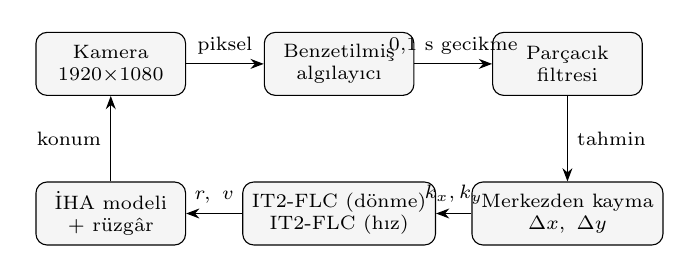
\begin{tikzpicture}[font=\scriptsize,
 box/.style={draw, rounded corners, minimum height=8mm, minimum width=19mm, align=center, fill=gray!8},
 >=Stealth]
\node[box] (cam) at (0,0) {Kamera\\1920$\times$1080};
\node[box] (det) at (2.9,0) {Benzetilmiş\\algılayıcı};
\node[box] (pf)  at (5.8,0) {Parçacık\\filtresi};
\node[box] (proj) at (5.8,-1.9) {Merkezden kayma\\$\Delta x,\ \Delta y$};
\node[box] (flc) at (2.9,-1.9) {IT2-FLC (dönme)\\IT2-FLC (hız)};
\node[box] (uav) at (0,-1.9) {İHA modeli\\+ rüzgâr};
\draw[->] (cam) -- node[above]{piksel} (det);
\draw[->] (det) -- node[above]{0,1 s gecikme} (pf);
\draw[->] (pf) -- node[right]{tahmin} (proj);
\draw[->] (proj) -- node[above]{$k_x,k_y$} (flc);
\draw[->] (flc) -- node[above]{$r,\ v$} (uav);
\draw[->] (uav) -- node[left]{konum} (cam);
\end{tikzpicture}
\caption{Benzetimdeki kapalı döngü. Makaledeki yapay zekâ modeli yerine gecikmeli ve gürültülü bir benzetilmiş algılayıcı kullanılmıştır.}
\label{fig:arch}
\end{figure}

Tablo~\ref{tab:params} benzetimin temel değerlerini ve nereden geldiklerini göstermektedir. ``M'' ile işaretlenenler makaleden alınmıştır; ``V'' ile işaretlenenler bizim varsayımımızdır ve ayar dosyalarından değiştirilebilir.

\begin{table}[t]
\centering
\caption{Benzetim değerleri (M: makaleden, V: varsayım)}
\label{tab:params}
\footnotesize
\setlength{\tabcolsep}{4pt}
\begin{tabular}{@{}lll@{}}
\toprule
Parametre & Değer & Kaynak \\
\midrule
Kontrol adımı / süre & 0,05 s (20 Hz) / 40 s & V \\
İHA yüksekliği & 10 m & V \\
Hız aralığı & $[-2,2]$ m/s & M (Denk. 4) \\
Dönme hızı aralığı & $[-\pi/3,\pi/3]$ rad/s & M (Denk. 3) \\
Komut gecikmesi (hız/dönme) & 0,3 / 0,2 s & V \\
Kamera çözünürlüğü & 1920$\times$1080 & M (Tablo 1) \\
Yatay görüş açısı & 84$^\circ$ & V (Phantom 4 Pro) \\
Piksel gürültüsü $\sigma$ & 5 px & V \\
Algılama gecikmesi & 0,1 s & V \\
Parçacık sayısı & 500 & V \\
PF ölçüm std & 0,2 m & V \\
Rüzgâr hızları & 4,9 / 9,6 / 12,1 m/s & M (Tablo 2) \\
Kalan rüzgâr katsayısı $\alpha$ & 0,04 & V \\
Giriş ÜF'leri & Tablo~\ref{tab:mf} & M \\
FOU $\delta$ / alt ÜF boyu & 0,05 / 0,8 & V \\
Yakalama yarıçapı / süresi & 0,5 m / 1 s & V \\
Ayar / test tekrarı & 10 / 30 & V \\
\bottomrule
\end{tabular}
\end{table}

\subsection{Bulanık kontrolcünün yazılması}
Bulanık mantık kodunu (üyelik fonksiyonları, Tip-2 küme, KM ve Nie--Tan) hazır bir kütüphane kullanmadan, okunabilir biçimde sıfırdan yazdık ve 41 birim testiyle doğruladık. Makalede olmadığı için kendimiz seçtiğimiz değerler şunlardır:
\begin{itemize}
\item 0--28 ölçeği $k=(u-14)/14$ formülüyle $-1$ ile $1$ arasına taşındı. $\Delta x$ için de $\Delta y$'nin üçgenleri kullanıldı.
\item Belirsizlik payı: üst ÜF üçgeni her iki yana $\delta=0{,}05$ kadar genişletildi, alt ÜF üçgeni aynı kadar daraltıldı ve yüksekliği 0,8 alındı.
\item En uçtaki NB ve PB kümeleri ``omuz'' biçiminde yapıldı; yoksa en uç hata değerinde hiçbir kural çalışmaz.
\item Çıkış kelimelerinin merkezleri: LB $[-1,-0{,}9]$, LS $[-0{,}55,-0{,}45]$, ZO $[-0{,}05,0{,}05]$, RS $[0{,}45,0{,}55]$, RB $[0{,}9,1]$.
\item Kurallar min t-normuyla, tip indirgeme KM ile yapıldı; komut $(y_l+y_r)/2$ olarak alındı.
\end{itemize}
Şekil~\ref{fig:curves} ortaya çıkan üçgenleri ve kontrolcünün giriş--çıkış eğrilerini göstermektedir. Burada ilginç bir bulgu vardır: Benchmark ve Ayar~2'de ``orta'' üçgeninin tepesi tam ortada olmadığı için, hata sıfırken bile kontrolcü küçük bir komut üretir (Benchmark için yaklaşık $+0{,}10$). Bu, İHA'nın aracı yakaladıktan sonra hep biraz kaymasına yol açar. Sadece Ayar~1 simetriktir.

\begin{figure*}[t]
\centering
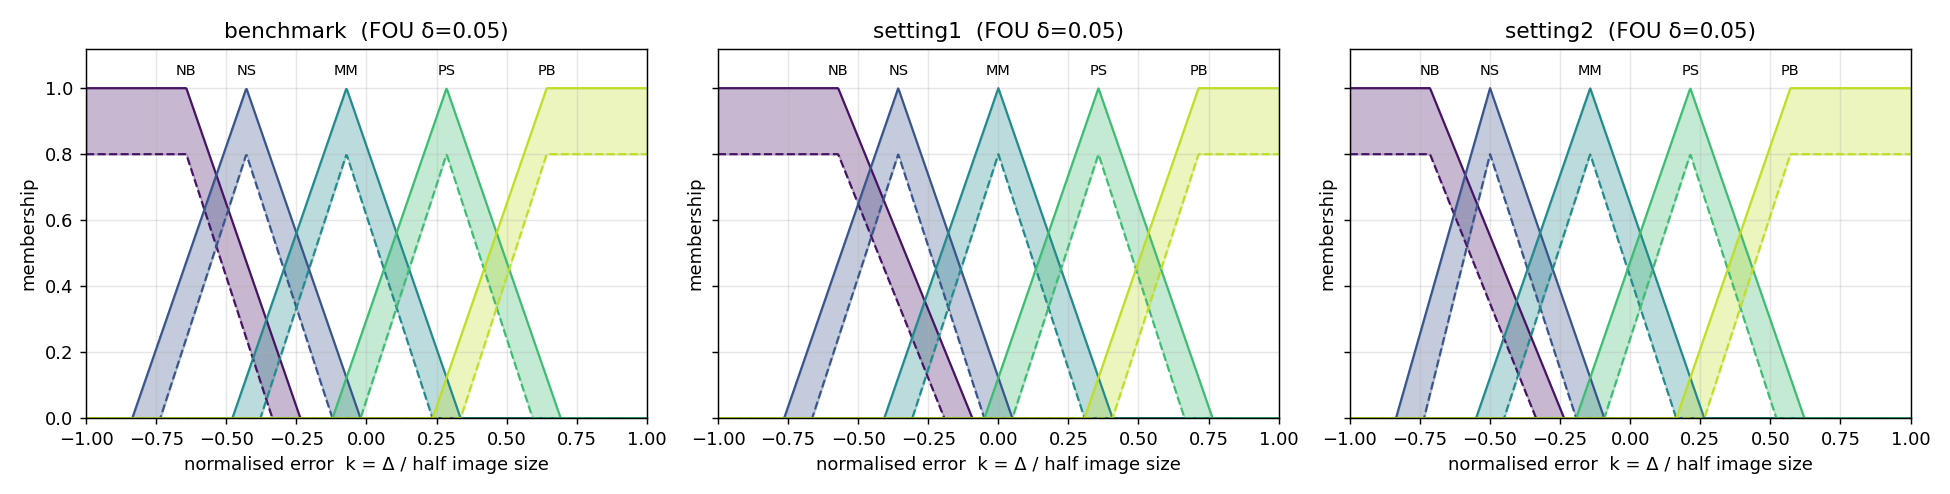
\includegraphics[width=0.95\textwidth]{mf_settings.png}\\[1mm]
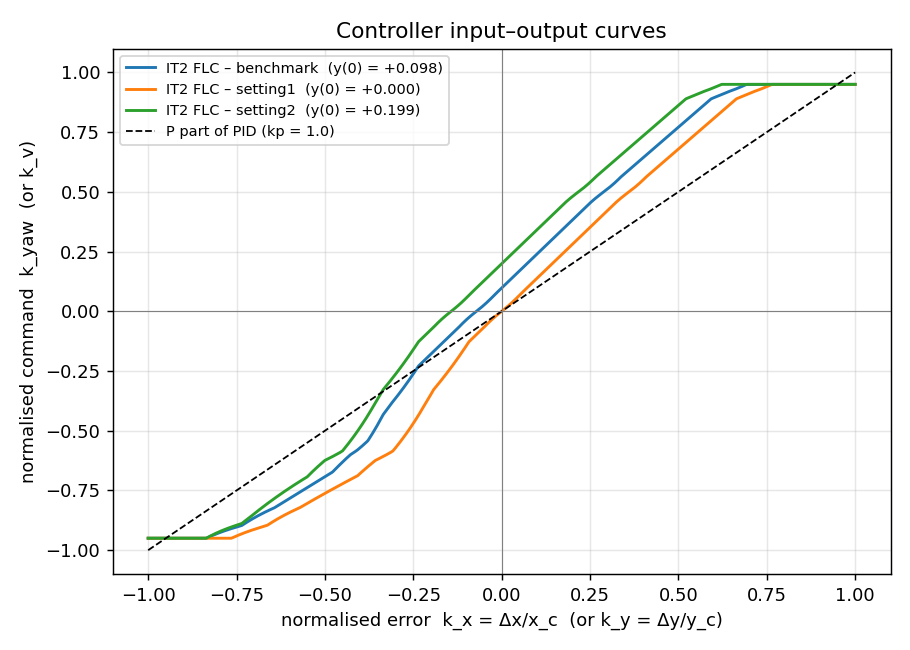
\includegraphics[width=0.42\textwidth]{control_curves.png}
\caption{Üstte: makaledeki üç üçgen ayarının Tip-2 hâli (gölgeli bölge FOU). Altta: kontrolcünün giriş--çıkış eğrileri; Benchmark ve Ayar~2 eğrileri sıfırdan geçmez.}
\label{fig:curves}
\end{figure*}

\subsection{Yazılımın yapısı ve tekrar üretilebilirlik}
Kod parçalara ayrılmıştır: \texttt{src/fuzzy/} bulanık mantık kodunu, \texttt{src/control/} PID'i, \texttt{src/sim/} İHA, kamera, araç, rüzgâr ve algılayıcı modellerini, \texttt{src/estimation/} parçacık filtresini, \texttt{src/metrics.py} ve \texttt{src/stats.py} ölçütleri ve istatistik testlerini içerir. Tüm ayarlar \texttt{configs/} klasöründeki YAML dosyalarındadır. Her deneme bir ``tohum'' sayısıyla başlatılır; aynı tohumu kullanan farklı kontrolcüler birebir aynı araç yolunu, aynı titremeyi ve aynı rüzgârı görür. Böylece karşılaştırma adil olur. Kullanılan paket sürümleri \texttt{requirements.txt} dosyasında sabitlenmiştir. Birim testleri üyelik fonksiyonlarını, KM'yi (ör. belirsizlik payı sıfırken sonucun Tip-1 ile aynı çıkması), yön işaretlerini, PID'i, ölçütleri ve benzetimi kontrol eder. Canlı gösterim için \texttt{demo/live\_demo.py} betiği, seçilen kontrolcüleri aynı denemede yan yana oynatır; araç hızı, rüzgâr, titreme ve kaybolma oranı komut satırından değiştirilebilir.

\subsection{Adil ayar yöntemi}
Makale PID'in ve bulanık kontrolcünün ayar değerlerini vermediği için bütün kontrolcüleri aynı yöntemle ayarladık: her kontrolcü için 60 farklı rastgele ayar denendi. Her ayar A, B ve C sahnelerinde 10 ayrı ``ayar tohumu'' (1000--1009) ile çalıştırıldı ve İHA ile araç arasındaki ortalama mesafeyi en küçük yapan ayar seçildi. PID için $k_p,k_i,k_d$; makale kontrolcüsü için giriş ve çıkış kazancı; önerilen kontrolcü için ek olarak türev kazancı ayarlandı. Bulunan değerler PID için $k_p=10{,}99$, $k_i=0{,}10$, $k_d=1{,}09$; makale kontrolcüsü için giriş kazancı 6,89, çıkış kazancı 2,83'tür. Sonuçların hepsi, ayarda hiç kullanılmamış 30 ``test tohumu'' (0--29) ile raporlanmıştır. Bu, makine öğrenmesindeki eğitim--test ayrımına benzer: kontrolcü sınav sorularını önceden görmez.

%======================================================================
\section{Önerilen Genişletme (Proposed Extension)}
\subsection{Neden?}
Makaledeki kontrolcünün tek girişi ve beş kuralı vardır; yalnızca ``araç nerede?'' sorusuna bakar. Hatanın büyüyüp büyümediğini, yani aracın uzaklaşıp uzaklaşmadığını bilmez. Kontrol dilinde bu, doğrusal olmayan bir P (oransal) kontrolcüdür. Oysa araç aniden yön değiştirdiğinde (C sahnesi) ya da hızla kaçtığında (A sahnesi) hatanın değişim hızı önemli bir bilgidir. Araba kullanırken fren yapmaya karar verirken de yalnızca öndeki araca olan mesafeye değil, ona ne hızla yaklaştığımıza da bakarız. Klasik kontrolde bu bilgi türev terimiyle (PD kontrolcü) eklenir; bulanık PD yapıları da literatürde iyi bilinmektedir~\cite{macvicar1976,kumbasar2014,sarabakha2018}.

\subsection{Tip-2 bulanık PD kontrolcü (IT2-FPD)}
Önerdiğimiz kontrolcünün iki girişi vardır: hata $e$ (makaledeki üçgenler hiç değiştirilmeden) ve hatanın değişim hızı $\dot e$. Piksel ölçümü titrek olduğu için türev doğrudan alınmaz; ardışık hataların farkı 0,1~s'lik bir yumuşatma filtresinden geçirilir. $\dot e$ için tepe noktaları $-1,-0{,}5,0,0{,}5,1$ olan beş simetrik Tip-2 üçgen kullanılır. İki giriş ve beşer kelime olduğu için $5\times5=25$ kural vardır. Kurallar, bulanık PD için klasik olan Mac Vicar-Whelan tablosundan alınmıştır~\cite{macvicar1976} (Tablo~\ref{tab:rules}): $(i,j)$ kuralının sonucu $\text{clip}(i+j-2,0,4)$ numaralı çıkış kelimesidir. Bu tablonun mantığı basittir: hata ve değişimi aynı yöndeyse hata büyüyordur, kontrolcü güçlü komut verir; zıt yöndeyse hata zaten küçülüyordur, kontrolcü yumuşak komut vererek hedefi aşmamaya çalışır. Hata için makalenin üçgenlerini koruduğumuzdan, gözlenen bütün farklar yalnızca eklediğimiz $\dot e$ girişinden gelir. Şekil~\ref{fig:surface} kontrolcünün iki girişe göre ürettiği komutu (kontrol yüzeyini) göstermektedir.

\begin{table}[t]
\centering
\caption{IT2-FPD kural tablosu (çıkış kelimeleri)}
\label{tab:rules}
\footnotesize
\begin{tabular}{@{}lccccc@{}}
\toprule
$e$ \textbackslash{} $\dot e$ & NB & NS & ZO & PS & PB \\
\midrule
NB & NB & NB & NB & NS & ZO \\
NS & NB & NB & NS & ZO & PS \\
MM & NB & NS & ZO & PS & PB \\
PS & NS & ZO & PS & PB & PB \\
PB & ZO & PS & PB & PB & PB \\
\bottomrule
\end{tabular}
\end{table}

\begin{figure}[t]
\centering
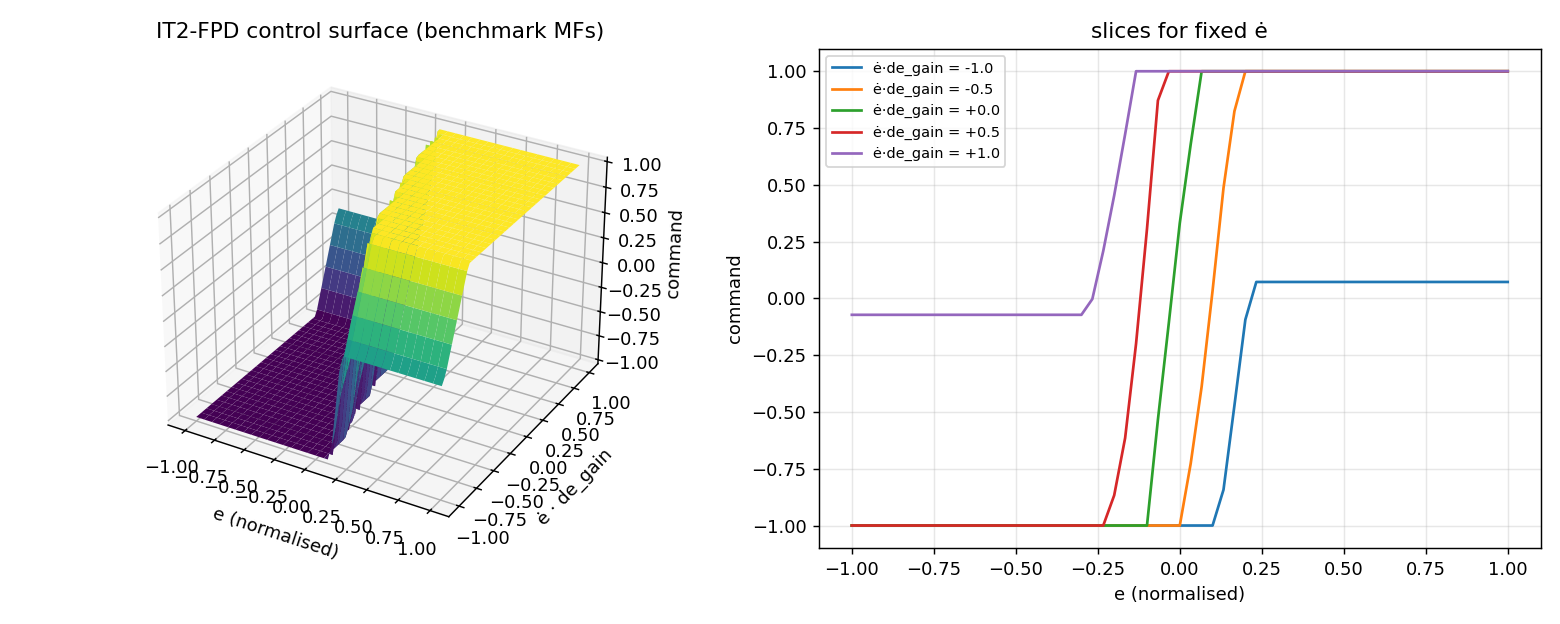
\includegraphics[width=\columnwidth]{ext_pd_control_surface.png}
\caption{Önerilen IT2-FPD'nin kontrol yüzeyi.}
\label{fig:surface}
\end{figure}

\subsection{Başarı ölçütü}
Önerilen kontrolcü, aynı ayar hakkıyla ayarlanmış makale kontrolcüsü ve PID ile aynı 30 test tohumunda karşılaştırılmıştır. Yakalama süresi, takip hatası ve gürbüzlükte istatistiksel olarak anlamlı bir iyileşme başarı sayılmıştır.

%======================================================================
\section{Deney Kurulumu (Experimental Setup)}
\textbf{Sahneler.} A: araç 1,6--2,0~m/s hızla düz gider ve ara sıra hafifçe döner. İHA'nın en yüksek hızı 2~m/s olduğu için bu, yakalanması zor bir hedeftir. B: araç 0,8--1,2~m/s hızla zikzak çizer; aracın görülemediği kareler \%20, yanlış tespitler \%3'tür; araç iki bölgede bir engelin altında kalır ve ışık değişimini temsil etmek için görüntü titremesi 5'ten 15 piksele çıkar. C: araç 10~s düz gider, sonra 2--5~s arayla 60--150$^\circ$ ani dönüşler yapar. Rüzgâr deneylerinde araç 1~m/s hızla düz gider.

\textbf{Ölçütler.} \emph{Yakalama süresi}: İHA ile araç arasındaki mesafenin ilk kez en az 1~s boyunca 0,5~m'nin altında kaldığı an; hiç yakalanamazsa 40~s yazılır. \emph{Takip hatası}: yakaladıktan sonra araçtan ortalama uzaklık. \emph{Gürbüzlük indeksi}: yakaladıktan sonraki uzaklığın standart sapması, yani İHA'nın ne kadar sallandığı (makaledeki tanım; düşük olan iyidir). Bunlara ek olarak yakalama oranı, deneme boyunca ortalama uzaklık, kontrol eforu ve adım başına hesaplama süresi de raporlanmıştır.

\textbf{İstatistik.} Her yöntem aynı 30 tohumla çalıştığı için sonuçlar çiftler hâlinde karşılaştırılabilir. Eşleştirilmiş $t$-testi ve Wilcoxon testi ile farkın şans eseri olma olasılığını ($p$ değeri) hesapladık; $p<0{,}05$ ise farkı anlamlı kabul ettik. Farkın büyüklüğünü Cohen $d_z$ ile ölçtük (kabaca 0,2 küçük, 0,5 orta, 0,8 büyük etki) ve \%95 güven aralıklarını verdik. Takip hatası, iki yöntemin de aracı yakaladığı denemeler üzerinden karşılaştırılmıştır.

\textbf{Deneyler.} R1: sahneler; R2: rüzgâr; R3: üçgen ayarları; E1: önerilen kontrolcü; E2: Tip-1 ve Tip-2; E3: belirsizlik payının genişliği; E4: görüntü titremesi ve kaybolma; E5: parçacık filtresi ve gecikme; E6: tip indirgeme yöntemi. Bütün tablo ve şekiller \texttt{python experiments/run\_all.py} komutuyla üretilir; bu rapordaki her sayı \texttt{results/tables/} klasöründeki dosyalardan alınmıştır.

%======================================================================
\section{Sonuçlar (Results)}
\subsection{Makale doğrulandı mı? Tip-2 kontrolcü ve PID}
Tablo~\ref{tab:repro} makalenin bildirdiği iyileşme ile bizim sonucumuzu karşılaştırmaktadır. Üç sahne birlikte değerlendirildiğinde Tip-2 bulanık kontrolcü, PID'e göre yakalama süresini \%10,3, takip hatasını \%12,6 azaltmıştır. Bu değerler, makalenin kendi Tablo~3'üne göre hesaplanan iyileşmeyle (\%12,5 ve \%9,3) aynı büyüklüktedir; özetteki \%19,2'den ise düşüktür. Saniye ve metre olarak değerler makaleden farklıdır, çünkü bizim deneylerimiz gerçek uçuş değil benzetimdir ve makale yakalama süresini nasıl ölçtüğünü tanımlamamıştır.

\begin{table}[t]
\centering
\caption{PID'e göre değişim: makale ve bu çalışma (A+B+C, 30 tohum)}
\label{tab:repro}
\footnotesize
\begin{tabular}{@{}lccc@{}}
\toprule
Ölçüt & Makale (özet) & Makale (Tablo 3) & Bu çalışma \\
\midrule
Yakalama süresi & $-19{,}2$\% & $-12{,}5$\% & $-10{,}3$\% \\
 & 5,2$\to$4,2 s & 4,8$\to$4,2 s & 17,01$\to$15,27 s \\
Takip hatası & $-15{,}0$\% & $-9{,}3$\% & $-12{,}6$\% \\
 & 0,80$\to$0,68 m & 0,75$\to$0,68 m & 0,886$\to$0,774 m \\
\bottomrule
\end{tabular}
\end{table}

Sahnelere ayrı ayrı bakıldığında (Şekil~\ref{fig:r1}) en büyük fark, görüntünün titrek olduğu ve aracın sık kaybolduğu B sahnesindedir: Tip-2 kontrolcü yakalama süresini \%22 ($p=0{,}029$, Wilcoxon $p=0{,}012$), takip hatasını \%28 ($p<0{,}001$, $d_z=-1{,}16$) azaltmıştır; yakalama oranı \%80'den \%90'a çıkmıştır. A sahnesinde yakalama süresi \%2,9 kısalmış ($p=0{,}015$), takip hatasındaki fark ise anlamlı değildir. C sahnesinde fark küçüktür; yalnızca deneme boyunca ortalama uzaklık \%3,1 düşüktür ($p=0{,}022$). Kısacası makalenin iddia ettiği üstünlük, özellikle gürültülü ortamda ortaya çıkmaktadır. Öte yandan hızlı araçta (A) Tip-2 kontrolcü PID'den daha çok sallanmaktadır (gürbüzlük 0,178 ve 0,093~m); bu da makalenin Tablo~3'teki gürbüzlük değerleriyle tutarlıdır.

\begin{figure*}[t]
\centering
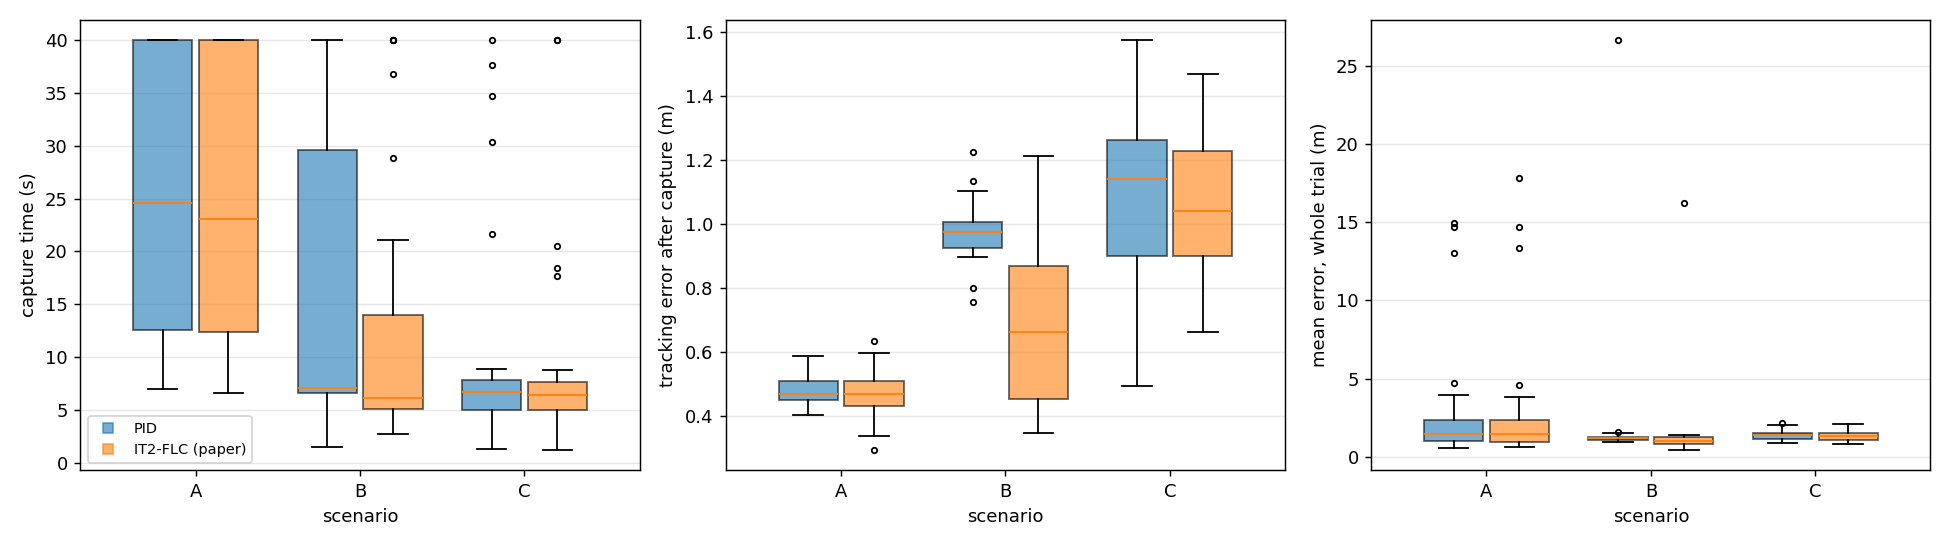
\includegraphics[width=0.95\textwidth]{repro_R1_scenarios.png}
\caption{R1: sahnelere göre PID ve makale kontrolcüsü (30 tohum, kutu grafikleri).}
\label{fig:r1}
\end{figure*}

Tablo~\ref{tab:r1stats} sahne bazındaki istatistik testlerini vermektedir.

\begin{table}[t]
\centering
\caption{R1 eşleştirilmiş testler: Tip-2 kontrolcü ile PID (negatif = Tip-2 daha iyi)}
\label{tab:r1stats}
\footnotesize
\begin{tabular}{@{}llrrrr@{}}
\toprule
Sahne & Ölçüt & $n$ & Değişim & $p$ ($t$) & $d_z$ \\
\midrule
A & Yakalama süresi & 30 & $-2{,}9$\% & 0,015 & $-0{,}47$ \\
A & Takip hatası & 20 & $-4{,}3$\% & 0,353 & $-0{,}21$ \\
B & Yakalama süresi & 30 & $-22{,}2$\% & 0,029 & $-0{,}42$ \\
B & Takip hatası & 23 & $-28{,}3$\% & $<$0,001 & $-1{,}16$ \\
C & Yakalama süresi & 30 & $-10{,}1$\% & 0,348 & $-0{,}17$ \\
C & Takip hatası & 28 & $-3{,}6$\% & 0,236 & $-0{,}23$ \\
C & Ort. uzaklık (tümü) & 30 & $-3{,}1$\% & 0,022 & $-0{,}44$ \\
\bottomrule
\end{tabular}
\end{table}

\textbf{Rüzgâr (R2).} Rüzgâr güçlendikçe her iki yöntemde de yakalama süresi ve hata artmaktadır (Tip-2 kontrolcü: rüzgârsız 4,66~s, 12,1~m/s'de 6,60~s). Fiziksel olarak beklenen budur; makalenin Tablo~2'sinde ise en güçlü rüzgârda en kısa süre bildirilmiştir. Rüzgârlı deneylerde Tip-2 kontrolcü aracı biraz daha hızlı yakalamakta (ör. 9,6~m/s'de 6,19 ve 6,44~s), PID ise yakaladıktan sonra araca biraz daha yakın durmaktadır (0,322 ve 0,369~m). Bunun olası nedeni, yukarıda değindiğimiz ``hata sıfırken bile küçük komut üretme'' durumudur.

\begin{figure*}[t]
\centering
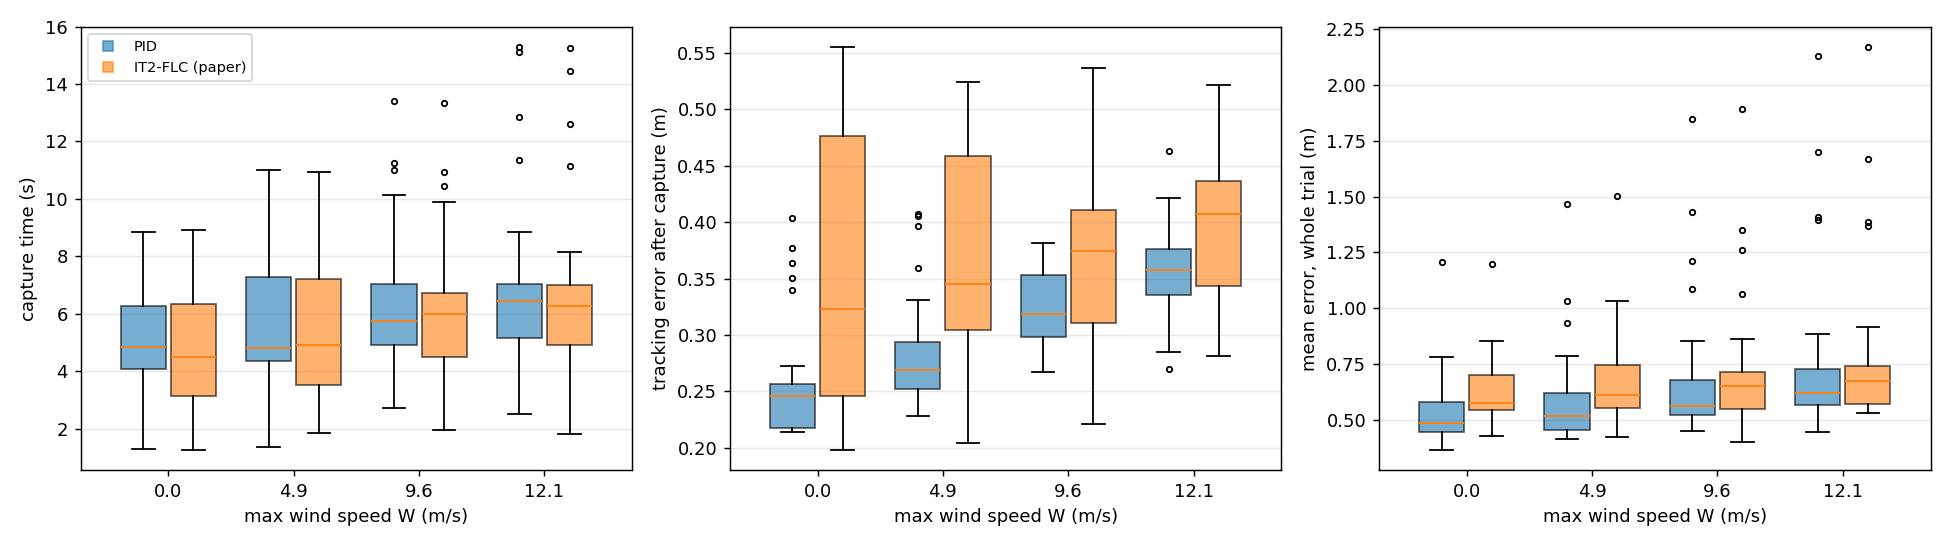
\includegraphics[width=0.95\textwidth]{repro_R2_wind.png}
\caption{R2: rüzgâr hızına göre PID ve makale kontrolcüsü (düz giden araç, ortalama ve \%95 güven aralığı).}
\label{fig:r2}
\end{figure*}

\textbf{Üçgen ayarları (R3).} Ayar~2 en düşük takip hatasını (0,731~m) ve en kısa yakalama süresini (14,43~s), Ayar~1 en yüksek takip hatasını (0,817~m) vermiştir. Makalede de en düşük hatayı Ayar~2 vermektedir (0,65~m). Üç ayar da PID'den (17,01~s, 0,894~m) daha iyidir.

\subsection{Önerilen IT2-FPD işe yaradı mı?}
Tablo~\ref{tab:ext} makale kontrolcüsü ile önerdiğimiz kontrolcüyü karşılaştırmaktadır. IT2-FPD daha az sallanmış (gürbüzlük \%10,4 daha iyi), deneme boyunca ortalama uzaklığı \%2,1, aracın görüntüden çıktığı süreyi \%8,1 azaltmıştır. Buna karşılık yakalama süresi \%13,9 uzamış, yakalama oranı \%84,4'ten \%76,7'ye düşmüş, takip hatası \%8 artmış ve hesaplama süresi \%45 artmıştır.

\begin{table}[t]
\centering
\caption{Makale kontrolcüsü ve önerilen IT2-FPD (A+B+C)}
\label{tab:ext}
\footnotesize
\begin{tabular}{@{}lccc@{}}
\toprule
Ölçüt & Makale & Önerilen & Değişim \\
\midrule
Yakalama süresi (s) & 15,27 & 17,38 & +13,9\% \\
Yakalama oranı (\%) & 84,4 & 76,7 & $-9{,}2$\% \\
Takip hatası (m) & 0,804 & 0,868 & +8,0\% \\
Gürbüzlük, std (m) & 0,452 & 0,405 & $-10{,}4$\% \\
Ortalama uzaklık, tüm deneme (m) & 1,982 & 1,940 & $-2{,}1$\% \\
Görüş dışı süre (\%) & 5,20 & 4,78 & $-8{,}1$\% \\
Kontrol eforu & 114,5 & 142,5 & +24,5\% \\
Çalışma süresi (ms/adım) & 0,672 & 0,975 & +45\% \\
\bottomrule
\end{tabular}
\end{table}

Sahnelere ayrı ayrı bakıldığında (Şekil~\ref{fig:e1}) tablo daha net görünür. Hızlı araçta (A) IT2-FPD açıkça kötüdür: yakalama süresi \%22 daha uzundur ($p<0{,}001$, $d_z=0{,}83$) ve yakalama oranı \%47'dir (makale kontrolcüsü \%70). Ancak aracı yakaladığında çok düzgün takip eder (gürbüzlük 0,071~m; makale kontrolcüsünde 0,178~m). Ani dönüşlü sahnede (C) IT2-FPD, 30 denemenin hepsinde aracı yakalayan tek yöntemdir ve yakalama süresi en kısadır (8,91~s); fakat makale kontrolcüsüne göre fark anlamlı değildir ($p=0{,}71$). PID'e göre ise C sahnesinde ortalama uzaklık \%5 daha düşüktür ($p<0{,}001$, $d_z=-1{,}06$) ve B sahnesinde takip hatası \%15 daha düşüktür ($p<0{,}001$). Rüzgâr deneyinde IT2-FPD en az sallanan yöntemdir (ör. 12,1~m/s'de 0,110~m; PID 0,148, makale kontrolcüsü 0,223~m), ancak takip hatası en yüksektir.

\begin{figure*}[t]
\centering
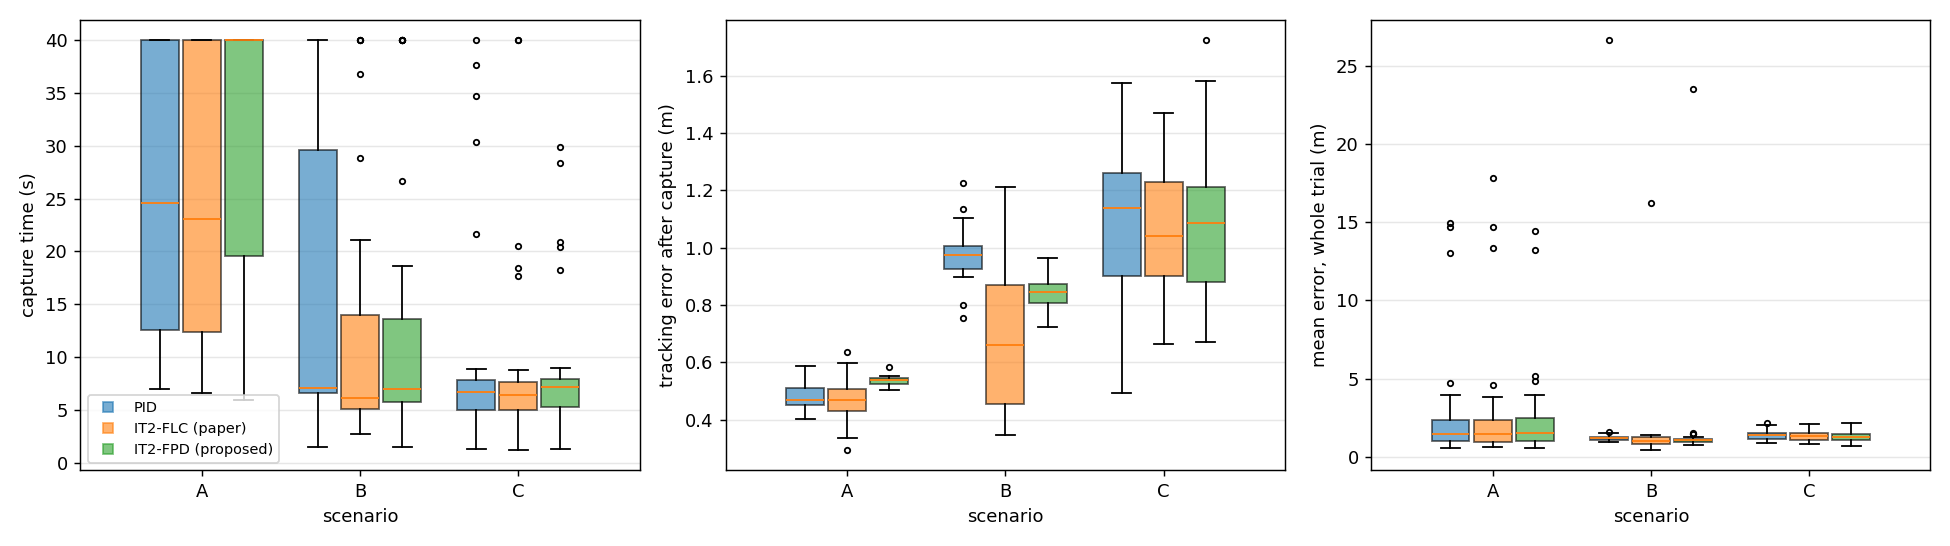
\includegraphics[width=0.95\textwidth]{ext_E1_scenarios.png}
\caption{E1: sahnelere göre PID, makale kontrolcüsü ve önerilen IT2-FPD.}
\label{fig:e1}
\end{figure*}

Şekil~\ref{fig:traj} aynı denemedeki örnek yolları göstermektedir: IT2-FPD araca daha az salınımla yaklaşmakta, ancak hızlı araçta geride kalmaktadır.

\begin{figure}[t]
\centering
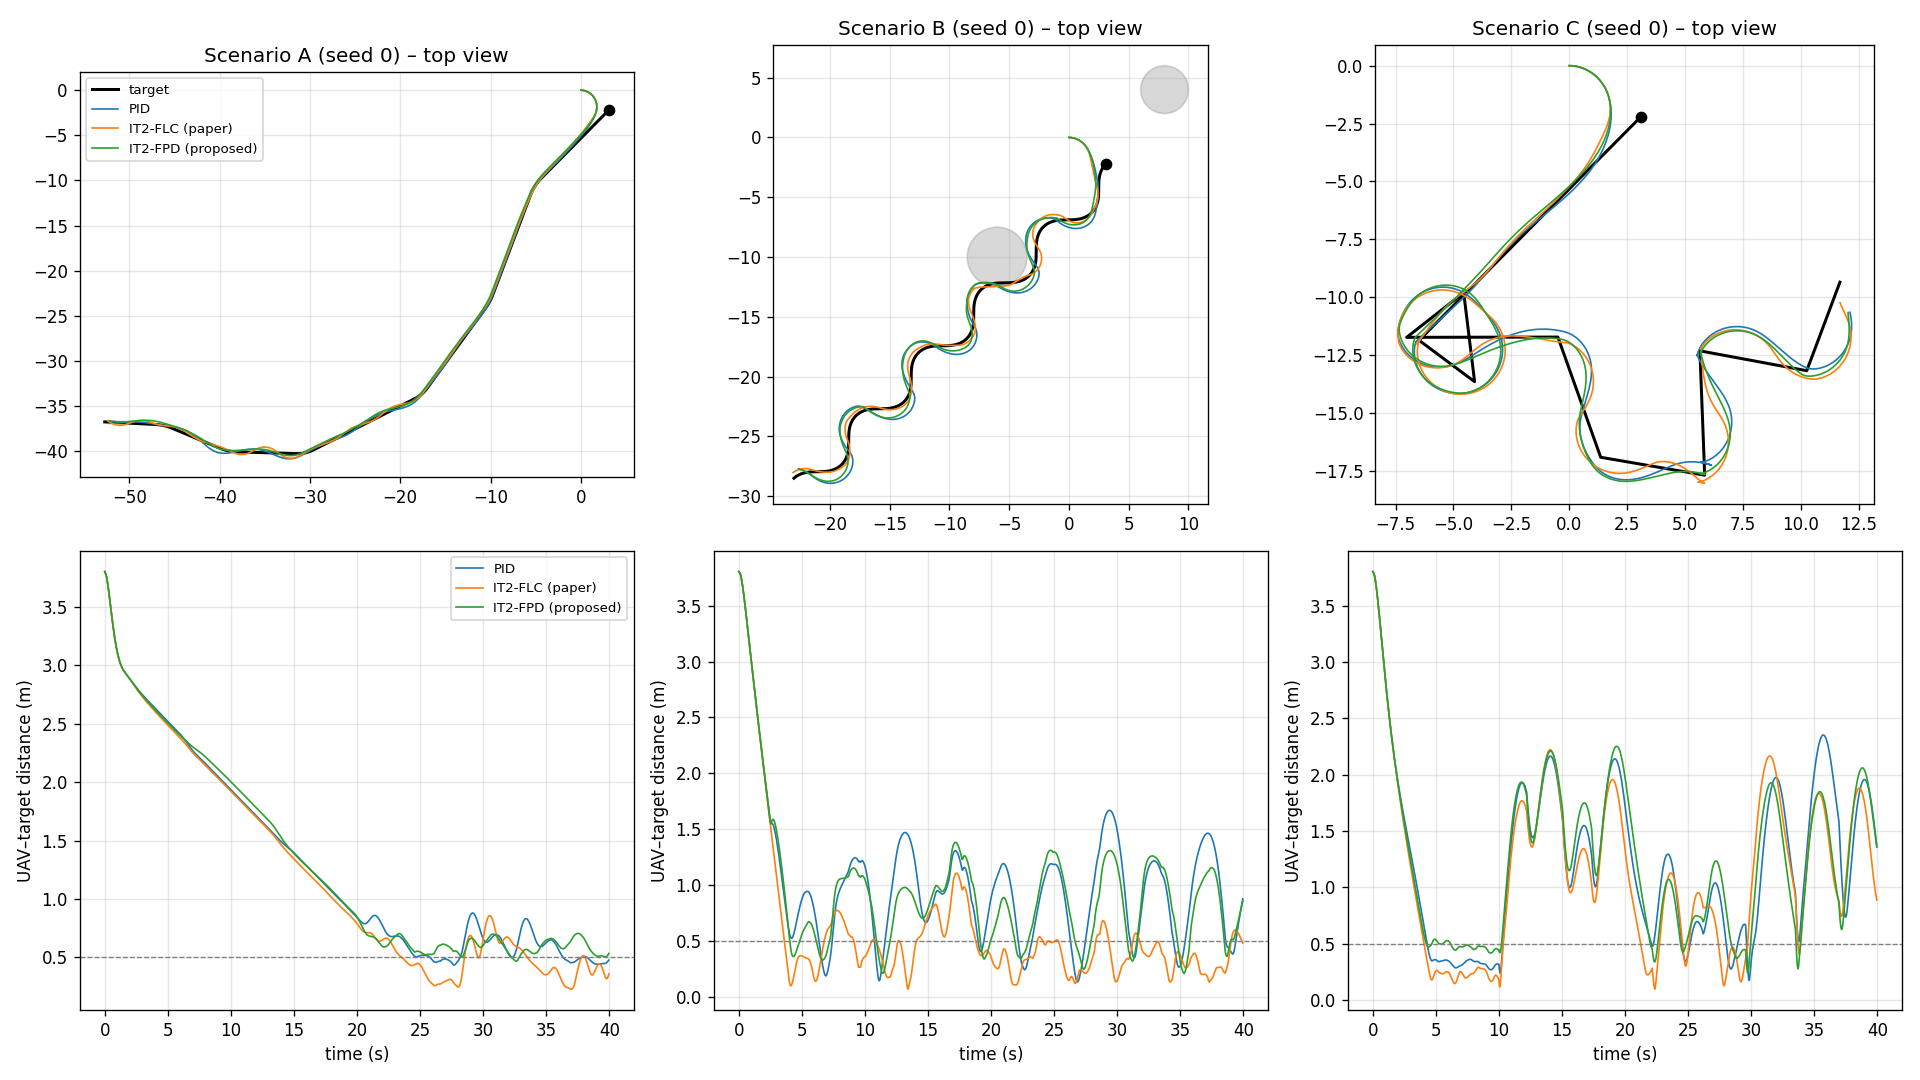
\includegraphics[width=\columnwidth]{ext_example_trajectories.png}
\caption{Aynı tohumda üç kontrolcünün örnek yolları (üstten görünüş).}
\label{fig:traj}
\end{figure}

\subsection{Ek deneyler: hangi parça neye etki ediyor?}
\textbf{Tip-1 mi, Tip-2 mi? (E2).} Belirsizlik payını kaldırıp kontrolcüyü Tip-1'e çevirdiğimizde makale kontrolcüsü hiçbir sahnede anlamlı olarak değişmemiştir (ör. A sahnesinde yakalama süresi 24,35 ve 24,35~s). Tek girişli ve beş kurallı bir yapıda belirsizlik payı, giriş--çıkış eğrisini çok az değiştirmektedir. Bizim IT2-FPD'de ise Tip-2, A sahnesinde yakalama süresini \%21 kısaltmış ($p<0{,}001$) ve yakalama oranını \%10'dan \%47'ye çıkarmıştır. Yani Tip-2'nin faydası, kontrolcünün girişi ve kuralı arttıkça ortaya çıkmaktadır. Bu, Wu'nun~\cite{wu2012} Tip-2 kontrolcülerin eğriyi duruma göre yumuşattığı bulgusuyla uyumludur.

\begin{figure*}[t]
\centering
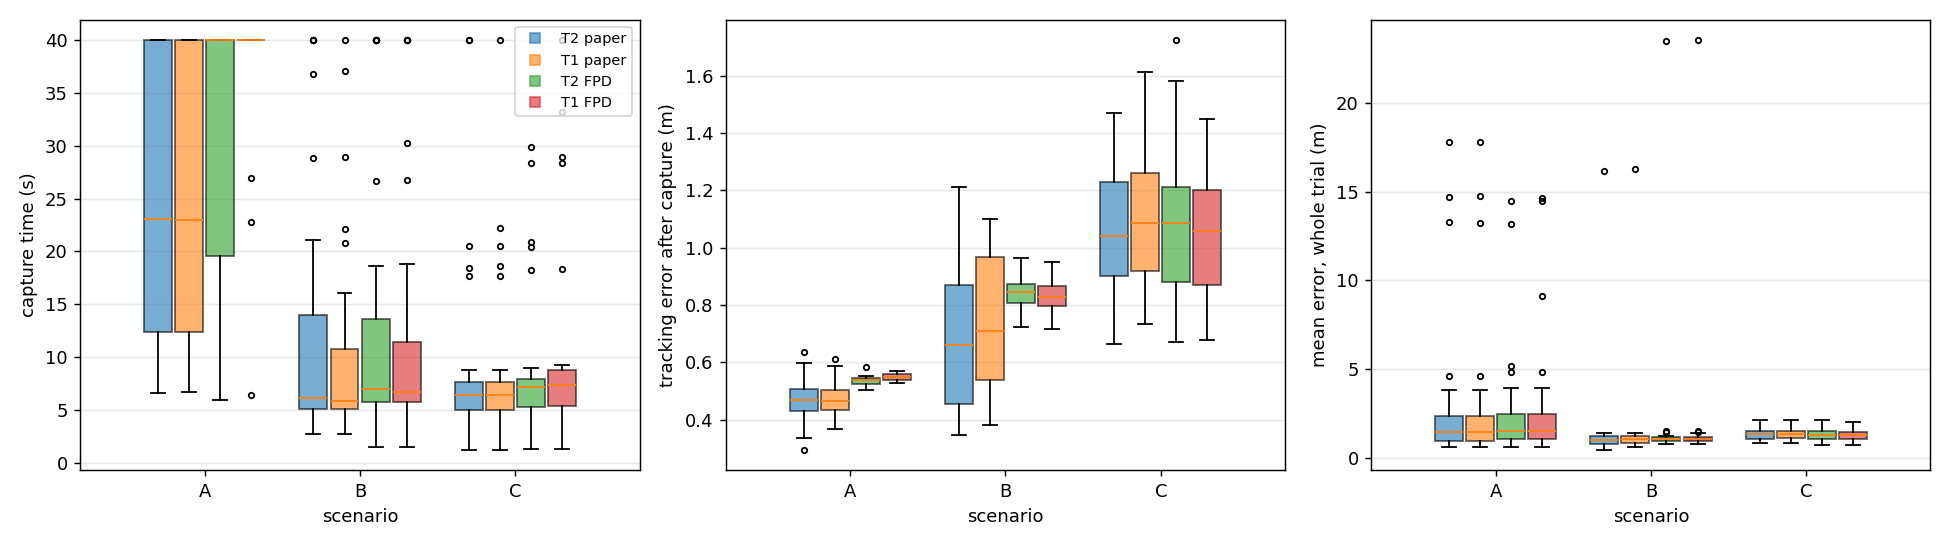
\includegraphics[width=0.95\textwidth]{ext_E2_t1_vs_t2.png}
\caption{E2: makale kontrolcüsü ve IT2-FPD için Tip-1 ile Tip-2 karşılaştırması.}
\label{fig:e2}
\end{figure*}

\begin{figure*}[t]
\centering
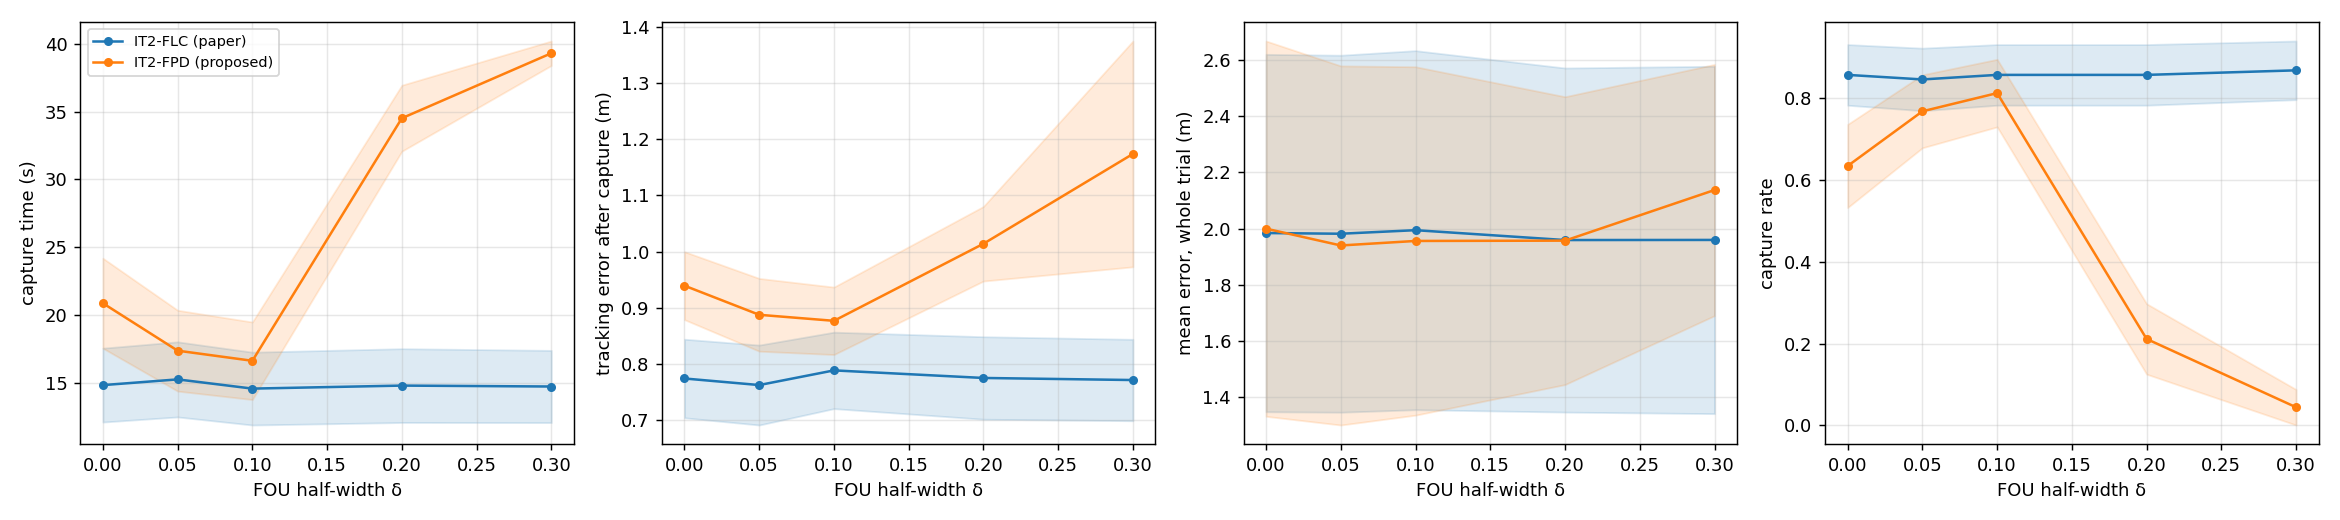
\includegraphics[width=0.95\textwidth]{abl_E3_fou.png}
\caption{E3: belirsizlik payının genişliğine ($\delta$) göre performans (A+B+C).}
\label{fig:e3}
\end{figure*}

\textbf{Belirsizlik payı ne kadar geniş olmalı? (E3).} Makale kontrolcüsü $\delta=0$--$0{,}3$ aralığında neredeyse hiç değişmemiştir (yakalama oranı \%84--87). IT2-FPD ise yalnızca küçük belirsizlik payında iyi çalışmaktadır: $\delta=0{,}1$'de yakalama oranı \%81 iken $\delta=0{,}2$'de \%21'e, $\delta=0{,}3$'te \%4'e düşmüştür. Geniş belirsizlik payı, türev girişinin etkisini bastırıp kontrolcüyü fazla yumuşatmaktadır.

\textbf{Görüntü titrer veya araç kaybolursa? (E4).} Piksel titremesi 40 piksele çıktığında makale kontrolcüsü \%50 yakalama oranını korurken PID \%10'a, IT2-FPD \%3'e düşmüştür (Şekil~\ref{fig:e4}). Bu, makalenin ``Tip-2 kontrolcü gürültüye dayanıklıdır'' iddiasını desteklemektedir. Türev, titremeyi büyüttüğü için IT2-FPD 20 pikselden itibaren hızla bozulmaktadır. Aracın görülmediği karelerin oranı \%40'a çıktığında ise, parçacık filtresi sayesinde hiçbir yöntem belirgin biçimde etkilenmemiştir.

\begin{figure*}[t]
\centering
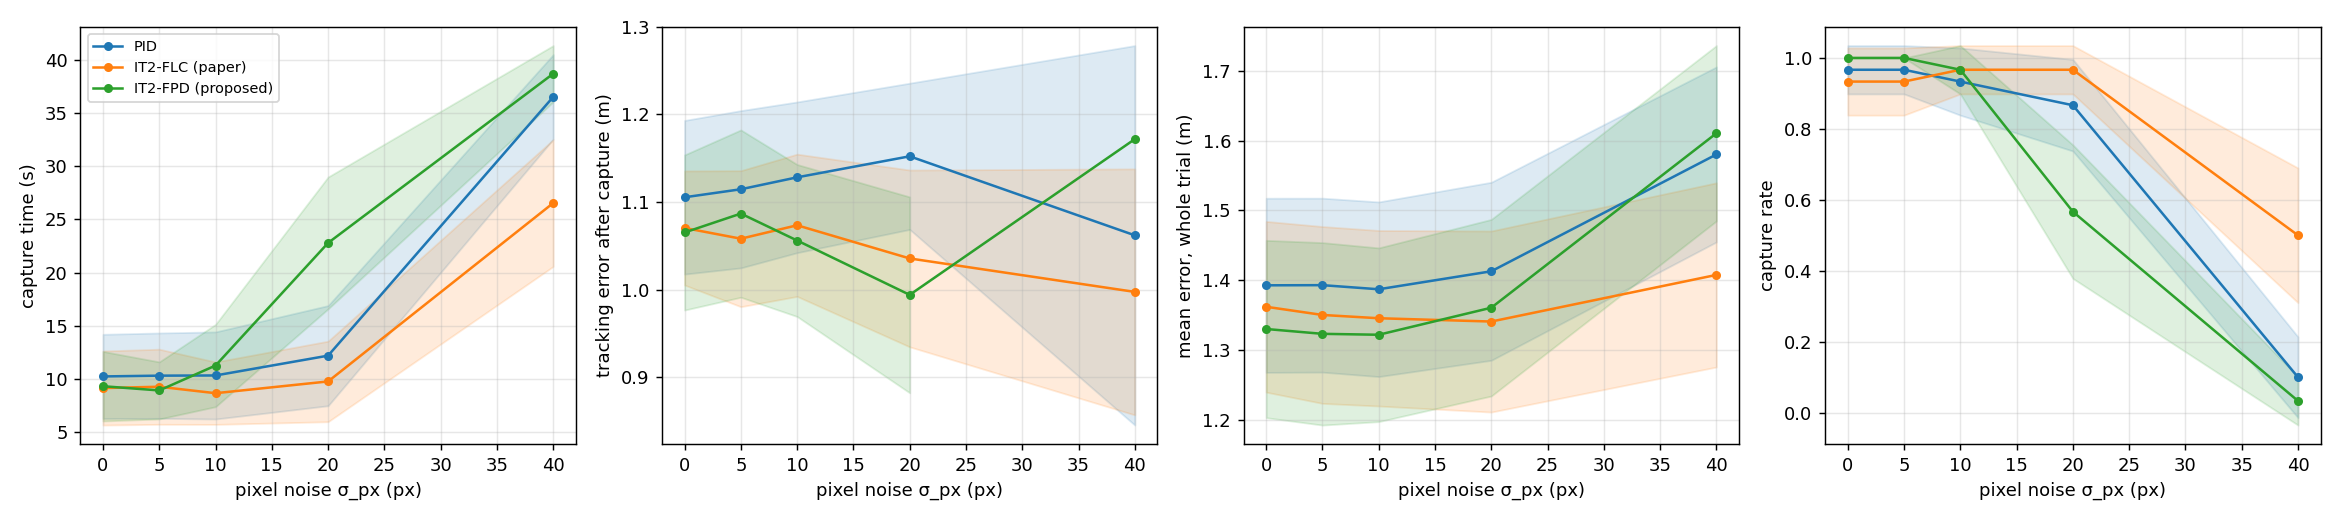
\includegraphics[width=0.95\textwidth]{abl_E4_sigma.png}
\caption{E4: piksel titremesine göre performans (C sahnesi).}
\label{fig:e4}
\end{figure*}

\textbf{Parçacık filtresi kapatılırsa veya gecikme artarsa? (E5).} Parçacık filtresi kapatılıp doğrudan en son ham ölçüm kullanıldığında IT2-FPD'nin yakalama oranı \%100'den \%50'ye, PID'inki \%97'den \%83'e düşmüş; makale kontrolcüsü ise \%93'te kalmıştır. Algılama gecikmesi 0,1'den 0,3~s'ye çıktığında takip hatası PID'de \%13, makale kontrolcüsünde \%10, IT2-FPD'de \%6 artmıştır.

\begin{figure*}[t]
\centering
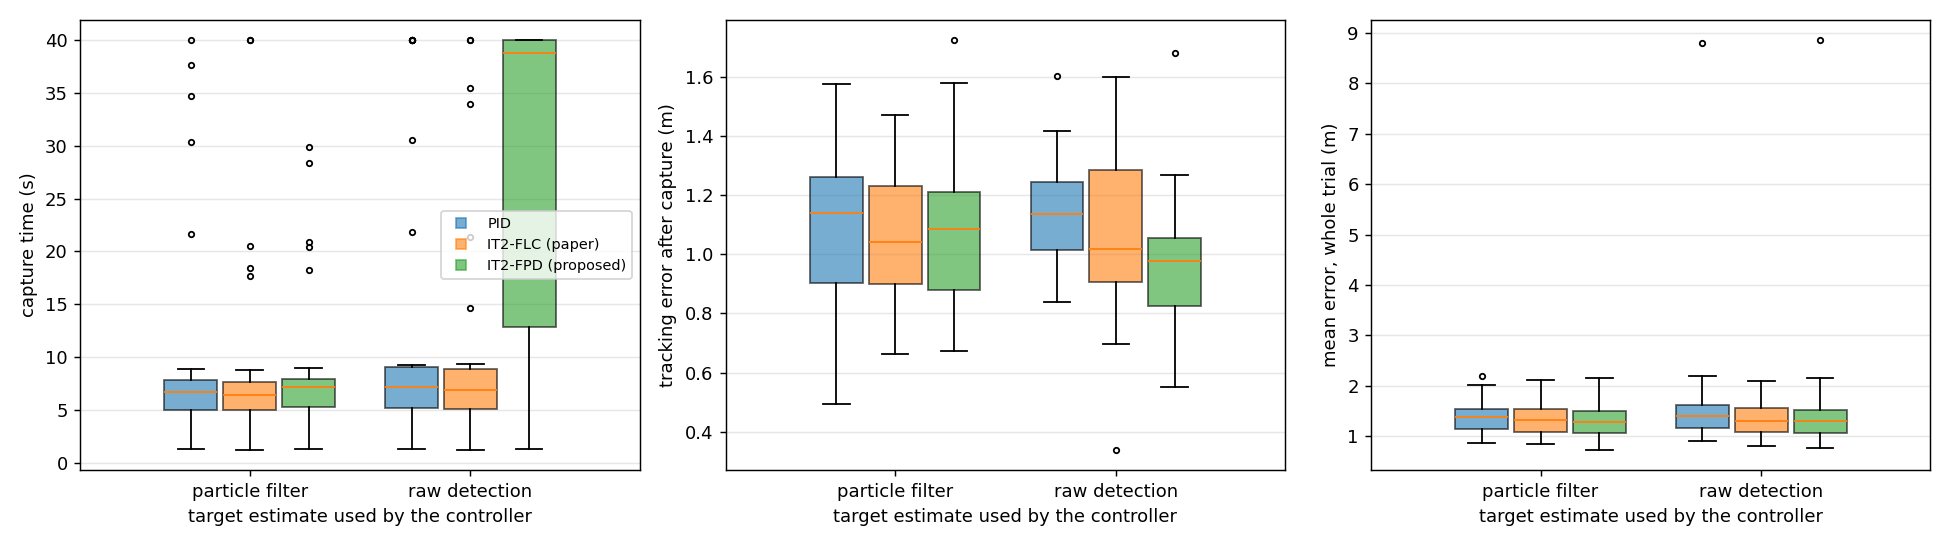
\includegraphics[width=0.95\textwidth]{abl_E5_pf.png}
\caption{E5: parçacık filtresi açık ve kapalı (C sahnesi).}
\label{fig:e5}
\end{figure*}

\textbf{Daha hızlı hesap yöntemi (E6).} Nie--Tan yöntemi, makale kontrolcüsünde KM ile aynı sonucu vermiş (C sahnesinde yakalama süresi 9,41 ve 9,26~s, $p=0{,}88$), ancak adım başına süreyi 0,71'den 0,31~ms'ye indirmiştir. IT2-FPD'de de süre 1,01'den 0,52~ms'ye inmiştir. Tüm Tip-2 kontrolcüler saniyede 20 komut (adım başına 50~ms) için fazlasıyla hızlıdır; PID ise 0,04~ms ile en hızlısıdır (Şekil~\ref{fig:e6}).

\begin{figure}[t]
\centering
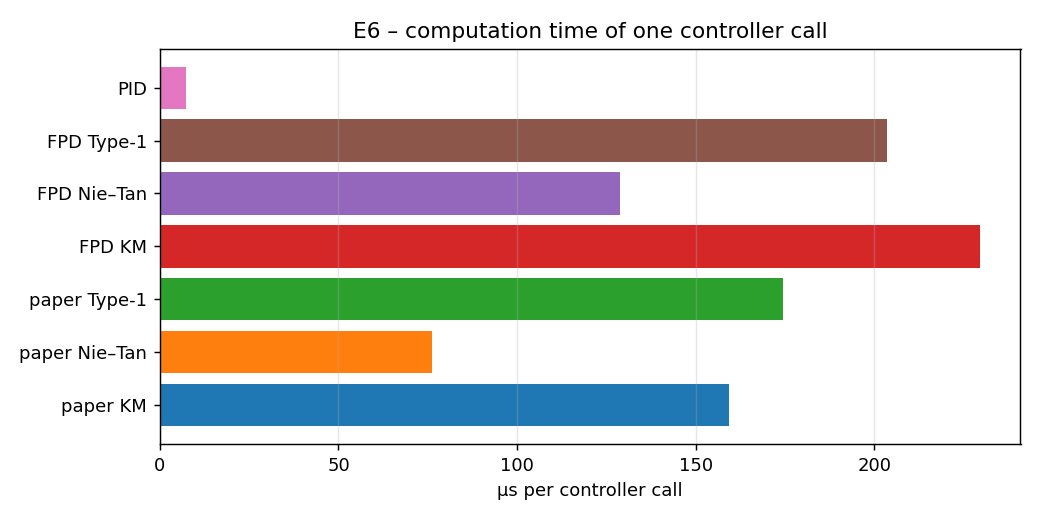
\includegraphics[width=\columnwidth]{abl_E6_compute_time.png}
\caption{E6: kontrolcü başına adım süresi (KM, Nie--Tan, Tip-1, PID).}
\label{fig:e6}
\end{figure}

%======================================================================
\section{Tartışma (Discussion)}
\textbf{Makale doğrulandı mı?} Makalenin ana iddiası, yani ``Tip-2 bulanık kontrolcü aracı PID'den daha hızlı yakalar ve daha az hatayla takip eder'' iddiası, PID'in de adil biçimde ayarlandığı bir benzetimde, makalenin Tablo~3'üne yakın bir büyüklükte doğrulanmıştır. Ancak kazanç her sahnede aynı değildir; çoğu gürültülü B sahnesinden gelmektedir. Özetteki \%20'lik iyileşme ise, özetteki PID sayısının aslında CNN'e ait olması nedeniyle abartılı görünmektedir.

\textbf{Önerdiğimiz kontrolcü neden daha iyi olmadı?} Türev girişi, İHA araca yaklaşırken hatanın küçüldüğünü görür ve komutu erkenden yumuşatır. Yavaş araçta bu iyidir: İHA hedefi aşmaz ve daha az sallanır (daha düşük gürbüzlük, C sahnesinde \%100 yakalama). Fakat A sahnesinde araç neredeyse İHA'nın en yüksek hızında gider; İHA'nın ona yetişmek için sürekli tam hızla gitmesi gerekir. Türev burada fren gibi davranır ve yakalamayı geciktirir. Ayrıca türev, görüntüdeki titremeyi büyüttüğü için yüksek gürültüde ve parçacık filtresi olmadan performans hızla düşer. Bu, klasik kontroldeki ``türev terimi gürültüye duyarlıdır'' bilgisiyle tutarlıdır. Türevi sadece hata büyükken devreye sokan bir yapı ya da aracın hızını parçacık filtresinden alıp önceden hesaba katan bir yapı daha uygun olabilir.

\textbf{Tip-2 gerçekten fark yaratıyor mu?} Makale kontrolcüsünde Tip-1 ile Tip-2 arasında anlamlı fark bulamadık. Makalenin belirsizlik payını tanımlamadığını da düşününce, makaledeki iyileşmenin Tip-2'den çok bulanık kontrolcünün doğrusal olmayan (yumuşak S biçimli) eğrisinden geldiği anlaşılmaktadır. Tip-2'nin katkısı ancak iki girişli ve 25 kurallı yapıda belirgin hâle gelmiştir.

\textbf{Hesaplama maliyeti.} KM tekrarlı çalıştığı için Nie--Tan'dan iki kat yavaştır, ama sonuca bir katkısı ölçülememiştir. Bu yüzden gerçek bir İHA'nın küçük bilgisayarında Nie--Tan tercih edilebilir.

%======================================================================
\section{Sınırlılıklar (Limitations)}
\begin{itemize}
\item Çalışma tamamen benzetimdir: İHA düz bir düzlemde hareket eder, gerçek uçuş ve gerçek görüntü işleme yoktur.
\item Rüzgâr modeli bir varsayımdır ($\alpha=0{,}04$); rüzgârın etkisinin büyüklüğü bu katsayıya bağlıdır.
\item Makalede verilmeyen birçok değer (belirsizlik payı, çıkış üçgenleri, $\Delta x$ üçgenleri, PID kazançları, parçacık filtresi ayarları) bizim seçimimizdir; hepsi gerekçeleriyle \texttt{docs/ASSUMPTIONS.md} dosyasında listelenmiştir.
\item Makaledeki CNN, DQN ve MPC karşılaştırmaları yeniden yapılmamıştır.
\item Ayar için rastgele arama kullanılmış ve 60 denemeyle sınırlandırılmıştır; daha fazla deneme sonuçları değiştirebilir.
\item Takip hatası yalnızca aracı yakalayan denemelerden hesaplandığı için, yakalama oranı düşük yöntemlerde (ör. A sahnesinde IT2-FPD) daha az denemeye dayanır.
\end{itemize}

%======================================================================
\section{Sonuç (Conclusion)}
Li vd.~\cite{li2024} tarafından önerilen Tip-2 bulanık mantık tabanlı İHA hedef takip yöntemini, tüm varsayımları açıkça yazılmış ve tek komutla yeniden çalıştırılabilen bir Python benzetiminde yeniden gerçekleştirdik. Tip-2 bulanık kontrolcünün PID'e göre yakalama süresini \%10,3, takip hatasını \%12,6 azalttığını ve bu üstünlüğün özellikle gürültülü ortamda belirgin olduğunu gösterdik. Makaledeki birkaç sayısal tutarsızlığı raporladık. Hata değişimini ikinci giriş olarak ekleyen IT2-FPD kontrolcümüz takibi daha düzgün hâle getirdi, ancak hızlı araçlarda yakalamayı geciktirdi ve gürültüye daha duyarlı oldu. Ek deneyler, Tip-2'nin faydasının çok girişli yapılarda ortaya çıktığını ve Nie--Tan yönteminin KM ile aynı doğrulukta yarı sürede çalıştığını gösterdi. Gelecekte türevin yalnızca büyük hatalarda devreye girdiği bir yapı, aracın hızını önceden hesaba katan bir ileri besleme ve gerçek bir İHA üzerinde deneme yapılması önerilmektedir.

%======================================================================
\section*{Üretken Yapay Zekâ Kullanım Beyanı (Generative AI Usage Disclosure)}
Bu çalışmada üretken yapay zekâ tabanlı bir kodlama asistanı; kodun yazımında, hata ayıklamada, belgelerin ve bu raporun taslağının hazırlanmasında ve kaynak künyelerinin kontrolünde yardımcı araç olarak kullanılmıştır. Tüm sayısal sonuçlar depodaki betiklerle üretilmiş, tüm kaynaklar DOI kayıtları üzerinden doğrulanmıştır. Yöntem seçimleri, sonuçların yorumu ve içeriğin doğruluğunun sorumluluğu yazara aittir.

%======================================================================
\begin{thebibliography}{99}
\bibitem{li2024} C. Li, W. Zhao, L. Zhao, L. Ju, and H. Zhang, ``Application of fuzzy logic control theory combined with target tracking algorithm in unmanned aerial vehicle target tracking,'' \emph{Sci. Rep.}, vol.~14, Art. no.~18506, 2024, doi: 10.1038/s41598-024-58140-5.
\bibitem{zadeh1965} L. A. Zadeh, ``Fuzzy sets,'' \emph{Inf. Control}, vol.~8, no.~3, pp.~338--353, 1965, doi: 10.1016/S0019-9958(65)90241-X.
\bibitem{mamdani1975} E. H. Mamdani and S. Assilian, ``An experiment in linguistic synthesis with a fuzzy logic controller,'' \emph{Int. J. Man-Mach. Stud.}, vol.~7, no.~1, pp.~1--13, 1975, doi: 10.1016/S0020-7373(75)80002-2.
\bibitem{macvicar1976} P. J. MacVicar-Whelan, ``Fuzzy sets for man-machine interaction,'' \emph{Int. J. Man-Mach. Stud.}, vol.~8, no.~6, pp.~687--697, 1976, doi: 10.1016/S0020-7373(76)80030-2.
\bibitem{karnik1999} N. N. Karnik, J. M. Mendel, and Q. Liang, ``Type-2 fuzzy logic systems,'' \emph{IEEE Trans. Fuzzy Syst.}, vol.~7, no.~6, pp.~643--658, 1999, doi: 10.1109/91.811231.
\bibitem{liang2000} Q. Liang and J. M. Mendel, ``Interval type-2 fuzzy logic systems: Theory and design,'' \emph{IEEE Trans. Fuzzy Syst.}, vol.~8, no.~5, pp.~535--550, 2000, doi: 10.1109/91.873577.
\bibitem{karnik2001} N. N. Karnik and J. M. Mendel, ``Centroid of a type-2 fuzzy set,'' \emph{Inf. Sci.}, vol.~132, no.~1--4, pp.~195--220, 2001, doi: 10.1016/S0020-0255(01)00069-X.
\bibitem{mendel2002} J. M. Mendel and R. I. B. John, ``Type-2 fuzzy sets made simple,'' \emph{IEEE Trans. Fuzzy Syst.}, vol.~10, no.~2, pp.~117--127, 2002, doi: 10.1109/91.995115.
\bibitem{nie2008} M. Nie and W. W. Tan, ``Towards an efficient type-reduction method for interval type-2 fuzzy logic systems,'' in \emph{Proc. IEEE Int. Conf. Fuzzy Syst.}, 2008, pp.~1425--1432, doi: 10.1109/FUZZY.2008.4630559.
\bibitem{wu2009} D. Wu and J. M. Mendel, ``Enhanced Karnik--Mendel algorithms,'' \emph{IEEE Trans. Fuzzy Syst.}, vol.~17, no.~4, pp.~923--934, 2009, doi: 10.1109/TFUZZ.2008.924329.
\bibitem{wu2012} D. Wu, ``On the fundamental differences between interval type-2 and type-1 fuzzy logic controllers,'' \emph{IEEE Trans. Fuzzy Syst.}, vol.~20, no.~5, pp.~832--848, 2012, doi: 10.1109/TFUZZ.2012.2186818.
\bibitem{hagras2004} H. A. Hagras, ``A hierarchical type-2 fuzzy logic control architecture for autonomous mobile robots,'' \emph{IEEE Trans. Fuzzy Syst.}, vol.~12, no.~4, pp.~524--539, 2004, doi: 10.1109/TFUZZ.2004.832538.
\bibitem{kumbasar2014} T. Kumbasar and H. Hagras, ``Big Bang--Big Crunch optimization based interval type-2 fuzzy PID cascade controller design strategy,'' \emph{Inf. Sci.}, vol.~282, pp.~277--295, 2014, doi: 10.1016/j.ins.2014.06.005.
\bibitem{sarabakha2018} A. Sarabakha, C. Fu, E. Kayacan, and T. Kumbasar, ``Type-2 fuzzy logic controllers made even simpler: From design to deployment for UAVs,'' \emph{IEEE Trans. Ind. Electron.}, vol.~65, no.~6, pp.~5069--5077, 2018, doi: 10.1109/TIE.2017.2767546.
\bibitem{harik2017} E. H. C. Harik, F. Guérin, F. Guinand, J.-F. Brethé, H. Pelvillain, and J.-Y. Parédé, ``Fuzzy logic controller for predictive vision-based target tracking with an unmanned aerial vehicle,'' \emph{Adv. Robot.}, vol.~31, no.~7, pp.~368--381, 2017, doi: 10.1080/01691864.2016.1271500.
\bibitem{zatout2022} M. S. Zatout, A. Rezoug, A. Rezoug, K. Baizid, and J. Iqbal, ``Optimisation of fuzzy logic quadrotor attitude controller -- particle swarm, cuckoo search and BAT algorithms,'' \emph{Int. J. Syst. Sci.}, vol.~53, no.~4, pp.~883--908, 2022, doi: 10.1080/00207721.2021.1978012.
\bibitem{dekoning2023} C. de Koning and A. Jamshidnejad, ``Hierarchical integration of model predictive and fuzzy logic control for combined coverage and target-oriented search-and-rescue via robots with imperfect sensors,'' \emph{J. Intell. Robot. Syst.}, vol.~107, no.~3, Art. no.~40, 2023, doi: 10.1007/s10846-023-01833-2.
\bibitem{tsitses2024} I. Tsitses, P. Zacharia, E. Xidias, and M. Papoutsidakis, ``A fuzzy-based system for autonomous unmanned aerial vehicle ship deck landing,'' \emph{Sensors}, vol.~24, no.~2, Art. no.~680, 2024, doi: 10.3390/s24020680.
\bibitem{gordon1993} N. J. Gordon, D. J. Salmond, and A. F. M. Smith, ``Novel approach to nonlinear/non-Gaussian Bayesian state estimation,'' \emph{IEE Proc. F Radar Signal Process.}, vol.~140, no.~2, pp.~107--113, 1993, doi: 10.1049/ip-f-2.1993.0015.
\bibitem{arulampalam2002} M. S. Arulampalam, S. Maskell, N. Gordon, and T. Clapp, ``A tutorial on particle filters for online nonlinear/non-Gaussian Bayesian tracking,'' \emph{IEEE Trans. Signal Process.}, vol.~50, no.~2, pp.~174--188, 2002, doi: 10.1109/78.978374.
\bibitem{chaumette2006} F. Chaumette and S. Hutchinson, ``Visual servo control. I. Basic approaches,'' \emph{IEEE Robot. Autom. Mag.}, vol.~13, no.~4, pp.~82--90, 2006, doi: 10.1109/MRA.2006.250573.
\bibitem{dosovitskiy2021} A. Dosovitskiy \emph{et al.}, ``An image is worth 16$\times$16 words: Transformers for image recognition at scale,'' in \emph{Proc. Int. Conf. Learn. Represent. (ICLR)}, 2021. [Online]. Available: \url{https://arxiv.org/abs/2010.11929}
\bibitem{nishad2025} D. K. Nishad, S. Khalid, D. Prakash, V. K. Singh, and P. Sahani, ``Advanced algorithms for UAV tracking of targets exhibiting start-stop and irregular motion,'' \emph{Sci. Rep.}, vol.~15, 2025, doi: 10.1038/s41598-025-13698-6.
\end{thebibliography}

\end{document}
